\documentclass[a4paper,12pt,english]{report}

\usepackage{babel}
\usepackage{hyperref}
\usepackage{graphicx}
\usepackage{listings}
\usepackage{appendix}

\usepackage{setspace}

\usepackage{color}
\usepackage{textcomp}
\definecolor{listinggray}{gray}{0.9}
\definecolor{lbcolor}{rgb}{0.95,0.95,0.95}
\lstset{
    backgroundcolor=\color{lbcolor},
    tabsize=4,
    rulecolor=,
    language=matlab,
        basicstyle=\scriptsize,
        upquote=true,
        aboveskip={1.5\baselineskip},
        columns=fixed,
        showstringspaces=false,
        extendedchars=true,
        breaklines=true,
        prebreak = \raisebox{0ex}[0ex][0ex]{\ensuremath{\hookleftarrow}},
        frame=single,
        showtabs=false,
        showspaces=false,
        showstringspaces=false,
        identifierstyle=\ttfamily,
        keywordstyle=\color[rgb]{0.1,0.1,0.6}\bfseries,
        commentstyle=\color[rgb]{0.133,0.545,0.133},
        stringstyle=\color[rgb]{0.627,0.126,0.941},
}

\usepackage{fancyhdr}
\pagestyle{fancy}
% \renewcommand{\sectionmark}[1]{\nouppercase\markleft{\thesection\ #1}}

\renewcommand{\chaptermark}[1]{\markright{\thechapter\ #1}}

\fancyhf{}
\fancyhead[R]{\bfseries\thepage}
\fancyhead[L]{\bfseries\rightmark}
% \fancyhead[LO]{\bfseries\rightmark}
% \fancyhead[RE]{\bfseries\leftmark}
\renewcommand{\headrulewidth}{0.5pt}
\renewcommand{\footrulewidth}{0.5pt}
\addtolength{\headheight}{5pt}
\addtolength{\footskip}{5pt}
\cfoot{\small A Framework for Small Distributed Projects and a Protein Clusterer Application}

\newcommand{\HRule}{\rule{\linewidth}{0.5mm}}
\newcommand{\fud}{\textbf{FuD}}
\newcommand{\fudepan}{\textbf{FuDePAN}}
\newcommand{\boost}{\textbf{boost}}

\renewcommand{\DJ}{\texttt{DistributableJob}}
\newcommand{\DJI}{\texttt{DistributableJobImplementation}}
\newcommand{\JU}{\texttt{JobUnit}}
\newcommand{\CP}{\texttt{ClientProcessor}}
\newcommand{\JM}{\texttt{JobManager}}
\newcommand{\CM}{\texttt{ClientsManager}}


\begin{document}

% \onehalfspacing

\pagenumbering{roman}

\begin{titlepage}
 
\begin{center}

%
\includegraphics[bb= 0 0 160 241]{/home/billy/unrc/proyecto_final/tesis/graficos/escudo.jpg}
%
\includegraphics[bb= 0 0 80 120]{images/escudo.jpg}
 
\textsc{\large Universidad Nacional de R\'io Cuarto \\ \normalsize Departamento de Computaci\'on}\\[2.9cm]
 
\textsc{\normalsize Proyecto Final}\\[0.2cm]
 
\HRule \\[0.4cm]
{ \Large \bfseries A Framework for Small Distributed Projects and a Protein Clusterer Application}\\[0.1cm]
\HRule 
\\[0.6cm]
{\normalsize 3 de Diciembre de 2009}
\vfill
\begin{minipage}{0.25\textwidth}
\begin{flushleft} \large
\emph{Author:}\\
Guillermo \textsc{Biset}
\end{flushleft}
\end{minipage}
\begin{minipage}{0.25\textwidth}
\begin{center} \large
\emph{Director:} \\
Marcelo \textsc{Arroyo}
\end{center}
\end{minipage}
\begin{minipage}{0.25\textwidth}
\begin{flushright} \large
\emph{Co-Director:} \\
Daniel \textsc{Gutson}
\end{flushright}
\end{minipage}
 
\end{center}
 
\end{titlepage}

\newpage

\begin{abstract} % \addcontentsline{toc}{chapter}{Abstract}
Computing on large data sets is an important part of computer science, a lot of important information is inherently difficult to compress and, additionally, the resources to process these amounts of data are usually expensive. Non-Profit Organizations, educational institutions and such must find ways to handle their processing requirements while keeping costs down. Several tools exist to accomplish this by means of some form of distributed computing.

This document provides overview of the design and implementation of an abstract framework to implement distributed algorithms independent of said tools, underlying communication systems or problem-specific concerns.
We consider this abstraction is necessary to maximize exploitation of available resources, a factor likely to change through time both in quantity and type.

The selected approach is a layered system containing application, management and distribution layers combining  server-client and Divide \& Conquer concepts to achieve high cohesion and low coupling while upholding the Open-Closed Principle.
The framework consists of fixed and variable parts, where the latter can be adapted to fit problem requirements by providing layer-specific details while inter operating with the static components and the rest of the system.
\end{abstract}

\newpage

\chapter*{Acknowledgements} \addcontentsline{toc}{chapter}{Acknowledgements}

% A Daniel Gutson, por su extrema dedicaci\'on a este proyecto, por ser todo lo que un mentor deber\'ia ser adem\'as de un gran amigo y ofrecerme desinteresadamente el m\'as preciado regalo que se puede recibir, conocimiento. Este trabajo es tan m\'io como suyo.

% A Rafael Garabato, Gustavo Domingo Yag\"uez y muchos otros relacionados a \fudepan \ que me ayudaron durante este emprendimiento. 

% A mis padres y familiares por ser una fuente inagotable de amor e inspiraci\'on y la fuerza motriz detr\'as de todos mis emprendimientos.

% A mi mejor mitad Ana por tenerme f\'e, por toda la ternura que la rodea, y a su familia por aceptarme y quererme como uno de los suyos.

% A Marcelo Arroyo y mis colegas y amigos del Departamento de Computaci\'on por todas las charlas estimulantes.

% A mis amigos todos y a la Pila, por su paciencia.

\newpage

\tableofcontents

\newpage

\listoffigures

\newpage

\listoftables

\newpage

\pagenumbering{arabic}

\part{Preliminaries}\label{prelim}

\chapter{Introduction}

%Motivation

Non-Profit Organizations (or NPO) usually lack large budgets or copious resources, so they need to maximize the use of available ones, a factor that can change both in type and quantity. On the other hand, in most fields of research data is much more abundant than processing power. This project started as a tool to develop a bioinformatic application for such an organization.

The framework here described attempts to provide starting ground for upcoming small to medium projects that need handling large data sets, particularly with high demands for stand-alone processing but low inter-node communication requirements independent of underlying implementation details regarding communication. 

It is imperative that the design of the framework allows the programmer of such a project to remain more concerned about the problem at hand rather than the underlying details such as where, when and how many resources will be available at any given moment.

%Goals

Many goals were taken into consideration while designing the framework, particularly to maintain flexibility at both ends of the design: first regarding the distributing middleware, e.g. BOINC, MPI, PVM, etc. and second concerning the problem to be implemented. On the other hand, fast prototyping capability (to test application code seamlessly) was needed and, finally, it was necessary to have well separated concerns throughout modules and aspects of the framework to achieve high cohesion and low coupling while upholding the Open-Closed Principle\cite{oosc}.

%This framework

The framework was originally designed to carry out the implementation of a data clustering\cite{clustering} algorithm on a large set of protein backbones using BOINC\footnote{\texttt{http://boinc.berkeley.edu/}} but eventually evolved to be used for most small distributed computing problems using different distributing middlewares.

%Other approaches

There is a great abundance of terms and classifications differentiating similar (but subtly different) situations of a distributed computer layout. These will be clarified in the following chapter, along with some examples and the cases taken into consideration herein.

Many approaches have been taken to allow programmers to focus on the problem rather than the distribution strategy and communication issues:
\begin{description}
 \item [BOINC] (or Berkeley Open Infrastructure for Network Computing\footnote{\texttt{http://boinc.berkeley.edu/}}) is a non-commercial middleware system designed at Berkeley for volunteer and grid computing\cite{boinc1}.
 \item [MPI] (or Message Passing Interface) is a specification for an API that allows many computers to communicate with one another\cite{mpi} that is mainly used throughout computer clusters and super computers.
 \item [OpenMP] (or Open Multi-Processing) is an application programming interface (API) that supports multi-platform shared memory multiprocessing programming\cite{openmp}.
 \item [MapReduce] is a programming model developed at Google to help the implementation of distributed algorithms without the input of the parallelization code itself\cite{mapreduce}.
\end{description}

One must note that these are not necessarily similar, BOINC is an actual application while \textbf{MPI} and \textbf{OpenMP} are only APIs with many different implementations. On the other hand, MapReduce is a model (but can also be considered an API if we don't fix the types) that can spur many different implementations.

This document introduces \fud\footnote{\texttt{http://fud.googlecode.com}}, a framework for work distribution. The acronym stands for \textbf{F}uDePAN \textbf{u}biquitous \textbf{D}istribution. The framework itself is a partially implemented library and can further use some or all of these approaches\footnote{However, the design itself will complicate the matters much if one were to try to apply OpenMP to implement message passing.}. 

\fud, when linked with a particular distributed middleware becomes an actual library. Later on, an application that uses this library is an actual program that solves a particular problem in a distributed manner. Currently \fud \ only supports a distributing middleware implemented with the Boost\footnote{\texttt{http://www.boost.org}} asynchronous input/output library\footnote{\texttt{http://www.boost.org/doc/libs/1\_40\_0/doc/html/boost\_asio.html}} (or \textbf{boost::asio}). A concise definition of \fud \ can be found in chapter \ref{fud}.

%This document

This document provides overview of said design and implementation details of the framework along with examples of its usage and some statistical results regarding performance and related issues. 

The document is divided into 4 parts. Part \ref{prelim} includes an introduction to this work, a chapter providing background to read the document and a review of the work methodology used to carry out the project. 

Part \ref{solution} is about the \fud \ framework, starting from the problem statement and the solution approach taken, here the reader will find details about both design and implementation of the framework along with simple examples of its usage. 

Part \ref{clusterer} introduces the protein clustering problem, considers many possible implementation and then goes on to explain how it was solved using the \fud \ framework.

Finally, part \ref{conclusions} brings to bear the conclusions drawn from the work and a road-map of the vast work that remains to be done.

In the Appendices part, there are two tutorials (one about building applications using \fud \ and another about extending \fud \ to use a different distributing middleware), two code metrics reports automatically generated and both the \fud \ and clusterer documentation. 

\chapter{Theoretical Background}

\section{Parallel Programming}

Parallel programming can be viewed as the study of algorithms and (collectively) programs that are executed on parallel computers. The term \emph{Parallel Computer} is to be taken under as broad interpretation as possible. In \cite{parallel} we have the following definition:

\begin{quote}
A  parallel computer is a set of processors that are able to work cooperatively to solve a computational problem. This definition is broad enough to include parallel supercomputers that have hundreds or thousands of processors, networks of workstations, multiple-processor workstations, and embedded systems. Parallel computers are interesting because they offer the potential to concentrate computational resources---whether processors, memory, or I/O bandwidth---on important computational problems. 
\end{quote}

However, it is possibly to classify the different possible computer layouts in order  to study the properties of each arrangement. In the following subsection we introduce the academic and industry standard taxonomy for such a purpose.

\subsection{Flynn's Taxonomy}

Flynn's taxonomy is a classification of computer architectures, proposed by Michael J. Flynn in 1966 and published in 1972\cite{flynn}. The classifications are based upon the number of concurrent instruction (or control) and data streams available in the architecture:

\begin{description}
\item [Single Instruction, Single Data stream] (or SISD): A sequential computer which exploits no parallelism in either the instruction or data streams. Examples of SISD architecture are the traditional uniprocessor machines like a PC or old mainframes. Figure \ref{sisd} shows an example diagram of this layout.
\begin{figure}[!ht]
\begin{center}
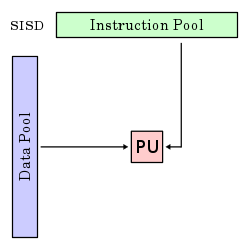
\includegraphics [bb= 0 0 200 200]{images/SISD.png}
\end{center}
\caption{Single Instruction Single Data diagram.}
\label{sisd}
\end{figure}
\item [Single Instruction, Multiple Data streams] (or SIMD): Used for a computer which exploits multiple data streams against a single instruction stream to perform operations which may be naturally parallelized. For example, an array processor or GPU. Figure \ref{simd} shows an example diagram of this layout.

\begin{figure}[!ht]
\begin{center}
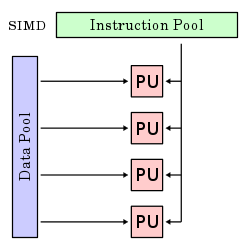
\includegraphics [bb= 0 0 200 200]{images/SIMD.png}
\end{center}
\caption{Single Instruction Multiple Data diagram.}
\label{simd}
\end{figure}

\item [Multiple Instruction, Single Data stream] (or MISD): Used when multiple instructions operate on a single data stream. Uncommon architecture which is generally used for fault tolerance. Heterogeneous systems operate on the same data stream and must agree on the result. Examples include the Space Shuttle flight control computer. Figure \ref{misd} shows an example diagram of this layout.

\begin{figure}[!ht]
\begin{center}
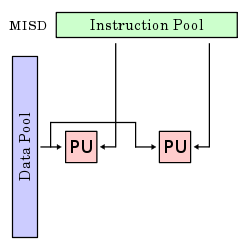
\includegraphics [bb= 0 0 200 200]{images/MISD.png}
\end{center}
\caption{Multiple Instruction Single Data diagram.}
\label{misd}
\end{figure}

\item [Multiple Instruction, Multiple Data streams] (or MIMD): Used when multiple autonomous processors simultaneously executing different instructions on different data. Distributed systems are generally recognized to be MIMD architectures; either exploiting a single shared memory space or a distributed memory space. Figure \ref{mimd} shows an example diagram of this layout.

\begin{figure}[!ht]
\begin{center}
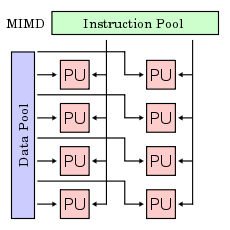
\includegraphics [bb= 0 0 200 200]{images/MIMD.png}
\end{center}
\caption{Multiple Instruction Multiple Data diagram.}
\label{mimd}
\end{figure}
\end{description}

The framework being presented here (\fud) has the capability of running in a MIMD computer layout with heterogeneous computers. The communication model, however,is a standard server/client organization, i.e. there will be exactly one server and 0 to many clients connected to it. More information can be found in section \ref{fud}. 

% \subsection{Asynchronous Computation}

% Async\cite{async}, 

% \subsection{Fault Tolerance}

% and Dijkstra\cite{faulttolerance}

\subsection{Load Balancing}

In computer networking, load balancing is a technique to distribute workload evenly across two or more computers, network links, CPUs, hard drives, or other resources, in order to get optimal resource utilization, maximize throughput, minimize response time, and avoid overload. Using multiple components with load balancing, instead of a single component, may increase reliability through redundancy. Usually, the load balancing service is provided by a dedicated program or hardware device.

Load balancing is commonly used to mediate internal communications in computer clusters, especially high-availability clusters or to implement scheduling algorithms for Operating Systems. 

In this last regard, \cite{sched2} has a good overview of scheduling algorithms and \cite{sched1} exhibits the implementation of a modern scheduling algorithm. Operating Systems design and its scheduling algorithms are extensively treated in Tanenbaum's books\cite{tanenbaum1} and \cite{tanenbaum2}.

Network load balancing, specifically regarding server implementations is thoroughly reviewed on \cite{loadbal}.

\subsection{BOINC}\label{boinc}

BOINC (Berkeley Open Infrastructure for Network Computing) is a platform for public-resource distributed computing. BOINC is being developed at U.C. Berkeley Spaces Sciences Laboratory by the group that developed and continues to operate SETI@home. BOINC is open source and is available at \texttt{http://boinc.berkeley.edu}\cite{boinc1}.

Many large scientific projects that require intensive computing employ the BOINC platform to fulfill their processing requirements. Among the more notable are:
\begin{description}
\item [SETI@home]: Performs digital signal processing of radio telescope data from the Arecibo radio observatory. A variety of interesting statistics and quantitative information regarding the BOINC project can be found in \cite{boinc2}.
\item [Predictor@home]: This project, based at The Scripps Research Institute, studies protein behavior using CHARMM, a FORTRAN program for macromolecular dynamics and mechanics.
\item [Folding@home]: Based at Stanford University, this project helps study protein folding, mis-folding, aggregation, and related diseases.
\item [Climateprediction.net]: Based at the Oxford University, the aim of this project is to quantify and reduce the uncertainties in long-term climate prediction based on computer simulations.
\end{description}

Also, BOINC supports an array of desirable features for large scale computing deployments\cite{boinc1}:
\begin{description}
\item [Redundancy computing]: A mechanism for identifying and rejecting erroneous results. These can spring because of malicious intentions on behalf of volunteers or some type of communication or computation problem.
\item [Failure and backoff]: To avoid overload of a server when trying to connect, clients will execute an exponential backoff scheme to avoid cluterring, i.e. they will delay reconnection proportionally to the number of connection failures.
\item [Participant preferences]: This mechanism allows participants (or volunteers) to select how and when their resources will be used via a number of configuration options.
\item [Credit and accounting]: BOINC provides an accounting system in which there is a unit of \emph{credit}, a wighted combination of computation, storage, and network transfer, which can be metered in various ways.
\item [User community features]: BOINC provides participant-oriented web sites features such as
\begin{itemize}
 \item The ability to form teams.
 \item he ability to create and browse 'user profiles' including text and images.
 \item Message boards and incorporation of a reputation system.
\end{itemize}
\item [Handling a large numbers of platforms]: To accommodate user privacy settings and other requirements, BOINC can be compiled and executed in a variety of different platforms.
\item [Graphics and screen-saver behavior]: Even though the core client appears monolithic, it is a combination of several components such as a \textbf{core client}, \textbf{client GUI}, the \textbf{API} and a \textbf{screen-saver}.
\item [Local scheduling]: A feature that allows the implementation of a \emph{policy} to define what job should be carried out next. Many factors weigh in to make this decision, such as project deadlines, hardware availability, etc.
\end{description}


\subsection{MapReduce}

MapReduce\cite{mapreduce} is a very interesting attempt at simplifying data processing on heterogeneous clusters. The approach is taken from simple functional programming techniques and comprise a couple of functions that represent the computation. These two functions are later automatically parallelized for a particular cluster layout.

MapReduce was developed at Google and their implementation was tailored for large clusters of commodity PCs connected together with switched Ethernet, but many different implementations are possible.

The advantage of this approach is simplicity, programmers (users of the programming model) must implement a pair of functions:
\begin{description}
\item [Map]: Takes an input pair and produces a set of intermediate key/value pairs. The implemented MapReduce library will later group together all intermediate values associated with the same intermediate key and pass them to the \emph{Reduce} function.
\item [Reduce]: This functions accepts an intermediate key and a set of values for that key. It then merges together these values to form a possibly smaller set of values. Typically just zero or one output value is produced per \emph{Reduce} invocation. The intermediate values are supplied to the user's reduce function via an iterator, which allows the implementer of the model to handle lists of values that are too large to fit in memory.
\end{description}


\section{Data Clustering}\label{dataclustering}

Loosely speaking, data clustering is the process of grouping objects together under some particular property. A proper definition and an extensive recount on clustering algorithms can be found on \cite{clustering}. From this same source we have the following definition:

\begin{quote}
Data clustering (or just clustering), also called cluster analysis, segmentation analysis, taxonomy analysis, or unsupervised classification, is a method of creating groups of objects, or clusters, in such a way that objects in one cluster are very similar and objects in different clusters are quite distinct.
\end{quote}

Of course, the notions of \emph{very similar} and \emph{quite distinct} are left to particular interpretation (i.e. its problem dependent). One may argue that objects in a particular cluster are only \emph{similar} (but not very) or that objects in different clusters are not really \emph{quite distinct}. Semantics and language play an interesting role when using words such as \emph{very} or \emph{quite} when coupled with abstract notions of similitude.

In the same literature, another (less ambiguous) definition can be found:

\begin{quote}
Roughly speaking, by data clustering, we mean that for a given set of data points and a similarity measure, we regroup the data such that data points in the same group are similar and data points in different groups are dissimilar.
\end{quote}

The key concept here is that there has to be a particular similarity measure in order to address the difference between data points. Of course a particular similarity measure could be just how different the data points are by some other definition.

To avoid confusion, one must separate the concepts of \textbf{distances} and \textbf{similarities}. In general, they are reciprocal concepts. Often, similarity measures and similarity coefficients are used to describe quantitatively how similar two data points are or how similar two clusters are: the greater the similarity coefficient, the more similar are the two data points. Dissimilarity measure and distance are the other way around: the greater the dissimilarity measure or distance, the more dissimilar are the two data points or the two clusters\cite{clustering}.

To look at an example, suppose that $\mathbf{x}$ and $\mathbf{y}$ are points in a $D$ dimensional space and $d$ is the function calculating the distance between two points in the standard Euclidean manner:

$$d(\mathbf{x},\mathbf{y}) = \left(\sum_{j=1}^{D}(\mathbf{x}_{j} - \mathbf{y}_{j})^{2} \right)^\frac{1}{2}$$

We could therefore use a similarity measure $m$ that is inversely proportional to $d$:

$$m = \frac{1}{d(\mathbf{x},\mathbf{y})}$$

It is interesting to see how the clusters might look while using this inversed similarity measure. However, no problems would arise in the use of this measure $m$ along with standard clustering algorithms. 

To illustrate the procudure of clustering, figure \ref{clusters}  shows a layout of two-dimensional points in a plane with three separate clusters (under aforementioned Euclidian definition of distance, not $m$).

Even though the terms \emph{cluster}, \emph{group} and \emph{class} have been used intuitively for the most part, it is possible to share some criteria to identify clusters and require objects in a cluster to:

\begin{enumerate}
\item share the same or closely related properties;
\item show small mutual distances or dissimilarities;
\item have ``contacts'' or ``relations'' with at least one other object in the group; or
\item be clearly distinguishable from the complement, i.e., the rest of the object in the data set.
\end{enumerate}

This lack of a formal notion of clustering could be irritating, but it will go away as soon as one is to tackle a particular clustering problem. It is therefore good to be ambiguous in the definition of \emph{cluster} since it will allow the use of the broad spectrum of clustering algorithms to a wide range of problems.

Each problem, in turn, will have a precise definition of how clusters should be formed and the previous ambiguity will be lost. In chapter \ref{clusterer} we show an interesting clustering problem and its implementation using the \fud \ framework.

There appear to be two ways of clustering numerical data: with compact clusters and chained clusters. A compact cluster is a set of data points in which members have high mutual similarity, it can usually be represented by a representative point or center. Figure \ref{clusters} shows such a case.

A chained cluster is a set of data points in which every member is more like other members in the cluster than other data points not in the cluster. Intuitively, any two data points in a chained cluster are reachable through a path. Figure \ref{clusters2} shows a case of two chained clusters, note that points in one cluster are closer to some points on the other cluster than to some of its own, however they are closer to at least one element in their same cluster.

\begin{figure}[!ht]
\begin{center}
\includegraphics [height=8cm]{images/clusters.eps}
\end{center}
\caption{Three well-separated center-based clusters in a 2D space.}
\label{clusters}
\end{figure}

\begin{figure}[!ht]
\begin{center}
\includegraphics [height=8cm]{images/clusters2.eps}
\end{center}
\caption{Two chained clusters in a 2D space.}
\label{clusters2}
\end{figure}

\subsection{Hard Clustering and Fuzzy Clustering}

In hard clustering, the results of the clustering algorithms can be represented by a partition on the data set $D$ (the conjunction of the members of the partition yields $D$ and pairwise intersection is non-empty).

In fuzzy clustering, the assumption is relaxed so that an object can belong to one or more cluster with probabilities. The result of fuzzy clustering algorithms can be represented by a $k \times n$ (where $k$ is the number of clusters and $n$ the number of records in the data set) matrix $U$ with the following constraints:
\begin{enumerate}
\item
$$u_{ji} \in (0,1], \qquad \qquad   1 \leq j \leq k, 1 \leq i \leq n$$
\item
$$\sum_{j=1}^{k} u_{ji} = 1, \qquad \qquad  1 \leq i  \leq n$$
\end{enumerate}

\subsection{Clustering Algorithms}

In general, conventional clustering algorithms can be classified into two categories: hierarchical algorithms and partitional algorithms. Hierarchical algorithms can either be divisive or agglomerative.

In a divisive hierarchical algorithm, the algorithm proceeds from the top to the bottom, i.e., it starts with one large cluster containing all data points and continues splitting clusters using some heuristic process.  Agglomerative hierarchical clustering is analogous, one starts with as many clusters as data points and then merges them under some rationale for doing so.

For large data sets, hierarchical methods become impractical unless other techniques are incorporated, because usually hierarchical methods are $O(n^2)$ for memory space and $O(n^3)$ for CPU time\cite{zait}, where $n$ is the number of data points in the data set.

Regarding partitional techniques, center based clustering algorithms are very efficient for clustering large databases. The goal of a center-based algorithm is to minimize its objective function, which define how good a clustering solution is.

\subsubsection{The \emph{k}-means algorithm}

The conventional \emph{k}-means algorithm described in table \ref{k-means} is one of the most used clustering algorithms. First described by Macqueen\cite{macqueen}, it was designed to cluster numerical data in which each cluster has a center called the mean.

Let $D$ be a data set with $n$ instances, and let $C_1$, $C_2$, \ldots, $C_k$ be the $k$ disjoint clusters of $D$. Then the error function is defined as

$$E= \sum_{i=1}^{k} \sum_{x\in C_i} d(\mathbf{x}, \mu (C_i))$$

where $\mu(C_i)$ is the centroid of cluster $C_i$, $d(\mathbf{x}, \mu (C_i))$ denotes the distance between $\mathbf{x}$ and $\mu(C_i)$ and it can be one of the many distance measures discussed before, a typical choice being the Euclidean distance defined before.

\begin{table}[!htb]
\lstset{language=Pascal}
\begin{lstlisting}[frame=single]
Require: Data set D, Number of clusters k, Dimensions d:
  {Ci is the ith cluster}
  {1. Initialization Phase}
1 : (C1,C2,...,Ck) := Initial partition of D.
  {2. Iteration Phase}
2 : repeat
3 :     dij := distance between case i and cluster j;
4 :     ni  := arg min 1<=j<=k dij;
5 :     Assign case i to cluster ni;
6 :     Recompute the cluster means of any changed clusters above;
7 : until no further changes of cluster membership occur
8 : Output Results
\end{lstlisting}
\centering \caption{The conventional \emph{k}-means algorithm.} 
\label{k-means}
\end{table}


\section{Proteins}\label{proteindefinition}

Proteins are polymers made of made of amino acids arranged in a linear chain. When dissolved in an aqueous, i.e. watery, environment they fold into globular form. The amino acids in the protein are joined together by the so-called peptide bonds. The sequence of amino acids in a protein is defined by the sequence of a gene, which is encoded in the genetic code. Figure \ref{geneticcode} shows how this encoding is accomplished.

Lehninger's book\cite{proteinsbook} has a thorough analysis on the subject of proteins and their importance to human health research.


\begin{figure}[!ht]
\begin{center}
\includegraphics [width=13cm]{images/Genetic_code.eps}
\end{center}
\caption{Genetic encoding.}
\label{geneticcode}
\end{figure}

Most proteins fold into unique 3-dimensional structures. The shape into which a protein naturally folds is known as its native conformation. Although many proteins can fold unassisted, simply through the chemical properties of their amino acids, others require the aid of molecular chaperons to fold into their native states. Biochemists often refer to four distinct aspects of a protein's structure:

\begin{description}
\item[Primary structure]: the amino acid sequence.
\item[Secondary structure]: regularly repeating local structures stabilized by hydrogen bonds. The most common examples are the alpha helix, beta sheet and turns. Because secondary structures are local, many regions of different secondary structure can be present in the same protein molecule.
\item[Tertiary structure]: the overall shape of a single protein molecule; the spatial relationship of the secondary structures to one another. Tertiary structure is generally stabilized by nonlocal interactions, most commonly the formation of a hydrophobic core, but also through salt bridges, hydrogen bonds, disulfide bonds, and even post-translational modifications. The term "tertiary structure" is often used as synonymous with the term fold. The Tertiary structure is what controls the basic function of the protein.
% \item[Quaternary structure]: the structure formed by several protein molecules (polypeptide chains), usually called protein subunits in this context, which function as a single protein complex.
\end{description}
\vspace{2.5cm} %GOD F%$#ING DAM*$#IT

\begin{figure}[!ht]
\begin{center}
% \includegraphics [bb= 0 0 380 380]{images/Myoglobin.png}
\includegraphics [bb= 0 0 380 380]{images/Myoglobin.jpg}
\end{center}
\caption{A cartoon representation of the 3D structure of myoglobin.}
\label{myoglobin}
\end{figure}

The amino acids in a polypeptide chain are linked by peptide bonds. Once linked in the protein chain, an individual amino acid is called a residue, and the linked series of carbon, nitrogen, and oxygen atoms are known as the main chain or protein backbone\cite{murrayetal}. Figure \ref{myoglobin} shows an example of a representation of the 3d structure of a protein.

% \begin{figure}[!ht]
% \begin{center}
% \includegraphics [bb= 0 0 354 241]{images/Peptide_bond.png}
% \end{center}
% \caption{Chemical structure of a particular peptide bond}
% \label{peptide}
% \end{figure}
% 
% \begin{figure}[!ht]
% \begin{center}
% \includegraphics [bb= 0 0 238 215]{images/Protein_repeating_unit.png}
% \end{center}
% \caption{Chemical structure of the peptide bond}
% \label{repunit}
% \end{figure}

\subsection{About Protein Clustering}

Several methods exist for protein clustering and classification. A summary about the most relevant methods can be found in \cite{proteinclustering}. 

Our particular concern is the clustering of many protein folds for a given backbone length. Most methods, however, were devised to classify variable protein data, i.e. from different proteins, whereas in our case we just want to cluster the same backbones.

More specifically, in our problem, the data set is a large collection of protein backbones, expressed in a sequence of atom positions (in a three dimensional space). Each data point then consist of the same number of 3d points. For example, a test database consist of 50000 possible backbone formations of a protein, each of which carries the position of 15 atoms.

\section{The C++ Programming Language}

C++ is a statically typed, free-form, multi-paradigm, compiled, general-purpose programming language. It is regarded as a middle-level language, as it comprises a combination of both high-level and low-level language features. It was developed by Bjarne Stroustrup starting in 1979 at Bell Labs as an enhancement to the C programming language and originally named ``C with Classes''. The most comprehensive reference for the language can be found in the great book by Stroustrup himself\cite{cplusplus}.

C++ was chosen as the implementation language because it allows for the use of Object Oriented techniques and produces extremely efficient machine code, resulting in fast programs. C++ also offers a plethora of libraries to choose from, allowing programmers to concentrate on the program at hand and not in reimplementing well known abstract data types.

As an example, consider the code excerpt from \fud \ in table \ref{cppfind}. Without going into an extensive explanation of what the code does, it is obvious to see that if it weren't for the intensive use of libraries, this code will look much more bloated or, otherwise, a careful implementation of the libraries used here would have been carried out.  

\begin{table}[!htb]
\lstset{language=C++}
\begin{lstlisting}[frame=single]
//exception if _ids_to_job_map[id] isn't defined
mili::find(_ids_to_job_map,id)->process_results(id, message);

//remove from pending list
std::list<JobUnit*>::iterator it;
it = find_if(_pendingList.begin(),_pendingList.end(), 
             boost::bind(&JobUnit::get_id, _1) == id);

if (it != _pendingList.end())
{
    delete *it;
    _pendingList.erase(it);
}
else
    syslog(LOG_NOTICE,"Finished JobUnit %u was not in pending list.",id);
\end{lstlisting}
\centering \caption{Excerpt \fud \ code to handle JobUnit completion.} 
\label{cppfind}
\end{table}

\chapter{Work Methodology}

\section{Software Practices}

The process of writing complex software is, at best, a complicated one. It has been compared to an engineering process, to the creation of mathematical formul\ae \ and even to artistic creation, to name a few. All of this comparisons on their own fall short of encompassing the true nature behind software development, nevertheless they all capture at least a part of the essence of software creation.

In an IBM web published article\cite{softwarepractices}, Mike Perks goes on to evaluate why most software projects fail and provides a summary of best practices for software development projects. Of the practices mentioned there, at least the following were implemented somewhat successfully:
\begin{description}
\item[Design]: During the development of \fud, at least half the time of the entire process was spent on design. Roughly speaking, about \%40 of the total time was used in the initial design stage (where no line of code was written). Later on, during implementation, many new modules were discovered and designed and old ones changed. Countless design decisions were either discarded or re-engineered.
\item[Code Construction]: Code changes and additions were integrated immediately, and tests were performed after a successful compilation of the code to check for major functional disruption. If the new or modified code passed this test, it was integrated to the repositories' trunk directory.
\item[Peer Reviews]: Most \emph{commit} operations on the code repository were reviewed by at least one person. Negative reviews included comments on specific changes in source files and these comments were then read by the implementer in order to either fix the problem or come to a mutual accord as to why the code should remain as before.
\item[Testing]: Testing is an integral part of software development. Throughout the development of \fud, several dummy applications were written to test different features of the framework. Each of these exposed one or more flaws in the system. Also, testing was done pro-actively, meaning that tests were devised before the actual code to be tested was written.
\item[Configuration Management]: Configuration management involves knowing the state of all artifacts that make up your system or project, managing the state of those artifacts, and releasing distinct versions of a system
\item[Issue Tracking]: Although not formally implemented, i.e. by the use of a particular tool, program errors (a.k.a. bugs) and other shortcomings were kept track of.
\end{description}

\section{Configuration Management}

To develop \fud \ it was necessary to keep track of several files of source code, an \textbf{svn} repository hosted at googlecode was used. Several repositories were used while the project evolved from a distributed clusterer application (using code of the framework to perform the distribution) to establishing the framework as a separate concept with the clusterer a single instance of an application that uses this framework.

A review of \textbf{Subversion}(svn) and its features can be found in O'Reilly's free book\cite{svn}, information about using GoogleCode can be found in its web page\footnote{\texttt{http://code.google.com/projecthosting/}}.

\section{Visual Aids and Models}

Throughout development, \textbf{UML} was used to communicate properties and structural information of the tools' design. Specification for \textbf{UML} can be found at Object Management Group's Homepage\footnote{\texttt{http://www.omg.org}} and several books exist about the subject from their authors\cite{uml}. As of this writing, the last version available can be downloaded from their download page\footnote{\texttt{http://www.omg.org/spec/UML/2.2/Infrastructure/PDF/}}.

For some information regarding dynamic properties of the system, a collection of Message Sequence Charts(sometimes referred to as \textbf{MSC}s) were used. They overcome some of the shortcomings in \textbf{UML} constructs regarding dynamic properties and object states.

\section{GNU/Linux and Free Software}

GNU/Linux is a wonderful free\footnote{\texttt{http://www.fsf.org}} Operating System under which all development of this project was undertaken. All other tools used to complete the project were free as well.

Freedom resides in the capability of analyzing and modifying the source code of the tool at hand. It is also possible to redistribute the work without any restrictions except keeping the license and maintaining references to the original authors. Therefore, this project aims to uphold these principles and is also published with these freedoms at hand.

The most popular free license at the moment is the \textit{GNU General Public License} (or \textbf{GPL}). A copy of the license used for this project can be found at \texttt{http://www.gnu.org/licenses/gpl-3.0.txt} and is also along the source code for the application.

\section{Tools}

On a side note, this work would not have been possible without the huge amount of excellent tools available under the nourishment of free software. Here is a short and incomplete list of the most used:

\subsection{GNU Toolchain}

Developing software in GNU/Linux is a fascinating endeavor, but this is partly because of the plethora of available tools for doing so. This project couldn't have been possible if it weren't for the GNU Toolchain, including (but not limited to) GNU make, gcc, gas, ld, and gdb.

\subsection{\LaTeXe}

This whole document was written using \LaTeXe, an extension of the original macro package \LaTeX {} (attributed to Leslie Lamport, see \cite{latex}) which, in turn, is based on \TeX, a program for typesetting text and mathematic formul\ae. \TeX was created by Donald Knuth in 1977\cite{texknuth}.

As a personal note, \LaTeXe {} is a crucial tool if aspiring to produce high quality scientific documents. Also, \LaTeXe is free (as usually is with good tools). A good summary of \LaTeXe capabilities and constructs can be found in \cite{tnssitl}.

\subsection{Editing}

\begin{description}
  \item [Kate:] A plain text editor\footnote{\texttt{http://kate-editor.org/}}.
  \item [Kile:] A \LaTeX {} editor based on  \textbf{kate}\footnote{\texttt{http://kile.sourceforge.net/}}.
\end{description}

\subsection{Graphics}

\begin{description}
  \item [Bouml:] A tool for \textbf{UML} diagrams\footnote{\texttt{http://bouml.free.fr/}}.
  \item [Gimp:] A tool for image handling\footnote{\texttt{www.gimp.org}}.
  \item [Dia:] A tool for general purpose diagrams\footnote{\texttt{http://live.gnome.org/Dia}}.
\end{description}

\subsection{Code Documentation}

\begin{description}
  \item [Doxygen:] A documentation system for C++, C, Java and many more languages\footnote{\texttt{http://www.doxygen.org}}.
\end{description}

\subsection{Static Code Analysis}

\begin{description}
  \item [Cloc:] A simple code line counting program\footnote{\texttt{http://cloc.sourceforge.net/}}.
  \item [CCCC:] A free software tool for measurement of source code related metrics\footnote{\texttt{http://cccc.sourceforge.net/}}.
  \item [GCov:] A  tool you can use in conjunction with GCC to test code coverage in your programs\footnote{\texttt{http://gcc.gnu.org/onlinedocs/gcc/Gcov.html}}.
\end{description}

\part{\fud}\label{solution}

\chapter{About \fud}\label{fud}

\section{Problem Statement}

The development of \fud \ originated from the need to implement a complex distributed algorithm on a large set of data for a Non-Profit Organization (\fudepan). 

Given that \fudepan \ depends on donated resources and that these can change through time, it wasn't possible to implement this algorithm specifically for a particular layout of the computers that were to do the processing, because such information was not (and could not be) available.

The idea arose to use some form of framework for automated work distribution. Immediately BOINC (see section \ref{boinc}) came to mind. But BOINC's architecture is not well suited for all types of layouts of processing nodes (i.e. high performance clusters).

However, the capability to use BOINC was a requirement, it would allow \fudepan \ to tap into an extremely rich supply of processing power volunteered by users\cite{boinc2}. But BOINC is a complex and large system and some of the applications that need to be implemented on \fudepan \ are small, their development with BOINC should prove to be a large effort for a simple problem. On the other hand, as possibilities of borrowing a high performance cluster became apparent, it was necessary to deal with them.

Thus, it was necessary to implement a framework for work distribution that could cover a large set of problems and could use different types of resources, without it being necessary to change the original implementation. We postulate that this was accomplished with the \fud \ design, but a lot of work (programming mostly) still remains in order to successfully exploit the genericity of the framework.

One limitation the \fud \ design was willing to concede was the one imposed on the size of the problems that should be implemented when using the framework. Large scale and complex problems that need volunteer support  should directly try using the BOINC framework (or similar) for their deployment. If, on the other hand, the project has vast resources at its disposal, then an implementation tailored to their available resources should be attempted.

Finally, \fud \ was developed to account for the following problem statement:

\begin{quote}
Design and develop a framework to automate the distribution of computational applications throughout a heterogeneous and dynamic layout of processing clients. The design should be flexible enough to allow programmers to use it to solve any computational problem while being able to use many distributing middlewares including (but not restricted to) BOINC and MPI. Finally, implementing an application shouldn't require the programmer to know parallel programming.
\end{quote}

Summarizing, \fud \ must be able to be used to solve any problem a sequential program can. Also, it must allow this without requiring the implementer to:
\begin{itemize}
\item Know parallel programming.
\item Depend on a particular layout of processing nodes.
\item Depend on a particular communication infrastructure.
\end{itemize}

Finally, \fud \ must ensure that:
\begin{itemize}
\item Your application has the potential to run parallely.
\item Your application will exploit all resources associated with it.
\item The framework won't impose severe performance drawbacks from its use.
\item Data exchanged between server and client applications won't carry a significant additional load on top of the original application's data.
\end{itemize}


\section{What is \fud?}

As stated before, \fud \ is a framework for work distribution, or a framework for the implementation of distributed applications. \fud \ doesn't depend on the problem that is to be implemented and doesn't force a particular communication model or any restrictions on the layout of the processing nodes it will use.

Therefore, \fud \ applications may run on heterogeneous and dynamic clusters. That is, the processing clients may vary in hardware and software properties, i.e. one could have many combinations of operating systems and hardware architectures running simultaneously. Also, the fact that the cluster is \emph{dynamic} means that processing clients may fault at any given time, their availability is not reliable either and so they may disconnect without previous warning or new clients may connect during the application's run time.

\fud \ itself is only a partially implemented library if the default distributing middleware (using boost::asio) is removed. However this middleware is bundled with the distribution of \fud \ and the framework can therefore be compiled as a library.

A compiled version of \fud \ comprises a library for work distribution using a particular distributing middleware. Libraries compiled with different middlewares should solve problems (execute the applications that use \fud) seamlessly, provided that client availability is not a problem in either middleware.

This last statement means that the same problem may be solved in a variety of computer clusters, even a single core computer running both the server and client applications together.

It is obvious, however, that different middleware implementations should try to benefit from the type of cluster layout that they are designed to handle. As an example, note the differences between MPI and BOINC, MPI is better suited for local clusters of interconnected computers (and usually share some type of fast interconnection). On the other hand, BOINC provides an extreme wealth of processing power\cite{boinc2}, but harnessing this power is done at the expense of Internet communication (which is much slower than an infiniband or some fast Ethernet configuration).

This modularity is exactly what was sought after when designing \fud. Non-Profit organizations usually don't have at their disposal high processing power capabilities and usually depend upon different types of contributions to handle their computational requirements.

\section{How does a \fud \ application work?}

In its broadest sense, \fud \ is divided into two applications: the server and the client. For any given \fud \ project, there must be exactly one server and number of clients connected to it. 

The server and its connected clients carry out a Master-Worker relationship, meaning that the server is in charge of the overall progress of the system and the workers (clients) are the ones making the bulk processing of data.

To understand how jobs are carried out, lets introduce first the basic terminology surrounding the project.

\subsection{Processing Clients}

A \CP \ is a processing node that is, somehow, connected to the server. Processing clients can take many forms and have different processing capabilities, so no assumptions should be made about how fast a client can handle data, its availability or any other characteristics.

The only task of a processing client is to wait for messages from the server. These messages will encapsulate some work that needs to be done. A client, however, won't know how this work might affect the rest of the system.

Once a client has a message it must process it and, once finished, inform that the results of the computation.

To illustrate this notion, figure \ref{master-worker} shows a server running a Clustering project (call it The Clusterer) that uses the \fud \ library with boosts asynchronous input output implementation to handle connections. In this case, there are two different types of operating systems connected to the server.

\begin{figure}[!ht]
\begin{center}
\includegraphics [width=11cm]{images/Master-Worker.eps}
\end{center}
\caption{Master Worker layout showing three connected clients.}
\label{master-worker}
\end{figure}

\subsection{Distributable Jobs}

A \DJ \ is an abstract work concept encapsulating any work that is to be performed. The notion is supposed to be taken as a \emph{large scale} job. There is no limit to the amount of distributable jobs there can be, nor to the type of any of them. 

It is possible that a complex project features many different types of distributable jobs, each of which will have many instances for different cases. The Clusterer, reviewed in section \ref{clusterer}, is an example of such a case.

The most important property of these large scale jobs is that they can be subdivided into smaller jobs (or Job Units, see next subsection) which will represent concrete computations to be carried out. 

A different way to put it is that there is no way to know beforehand how many job units will a distributable job produce in its lifetime\footnote{It's even possible that it will generate none.}. On the other hand, a job unit will represent a concrete computation.

From the distributable job's perspective, a couple of things are important about the job units he generated:
\begin{enumerate}
\item Even though generated in a given order, there shouldn't be any requirement as to the order the job units should be computed.
\item No two job units should represent the same computation, \fud \ will make sure that each generated job unit is eventually taken care of\footnote{Some implementations will even allow for redundancy checking on a job unit.}.
\end{enumerate}

So, the relationship between distributable jobs and job units is that of sub-tasking. But there are only these two levels, job units cannot be further subdivided and distributable don't represent a concrete list of computations to solve a problem.

As an example, consider diagram \ref{sumnvectors}. The example shows how someone could build an application to add the sum of $N$ vectors. Consider we have vectors $1$ through $N$, each having a variable amount of elements, and we need to obtain the sum of all the sums of elements in each vector. 

It is easy to see that only one type of distributable job is needed: one that can carry out the addition of a vector. We will then reuse this distributable job to compute the sum of all the partial sums by inserting each of them into a temporary vector $\mathbf{T}$.

It is important to note that there are many possibilities for synchronization here, but we will choose a simple one:
\begin{enumerate}
 \item Steps 1 and 2 will be executed concurrently. At any given moment, all connected clients could be processing different sections of different vectors.
 \item Step 3 will only commence once distributable jobs $1$ through $N$ are completed, at this point we now that vector $\mathbf{T}$ has all the partial results needed  to carry out the last vector sum, that of $\mathbf{T}$. At this point we will create distributable job $N+1$ with $\mathbf{T}$ as its parameter. When this distributable job is completed, we will have the total sum available.
\end{enumerate}

\begin{figure}[!ht]
\begin{center}
\includegraphics [width=10.2cm]{images/SumNvectors.eps}
\end{center}
\caption{Process of adding the sum of $N$ vectors.}
\label{sumnvectors}
\end{figure}

\clearpage

\subsection{Job Units}

A \JU \ is an abstract work concept encapsulating a simple task to be performed. This task comprises a particular list of steps to be carried out on a particular set of data.

A \JU \ is atomic, therefore it cannot be subdivided into other job units. The task itself must be represented by a message, which will later be passed on to a processing client to be computed. 

An important characteristic of job units is their size. There are two ways of looking at sizes, one is application defined (i.e. its interpretation depends on the application's problem) and the other is the actual size (e.g. in bytes) of the message it carries.

The sizes of job units may vary for many reasons. However, an important rule of thumb regarding sizes should be taken into consideration when generating one:
\begin{enumerate}
 \item Its actual size (i.e. the amount of bytes they occupy in memory) shouldn't be too large that they would clog an Internet communication channel.
 \item Its user-defined size shouldn't be too large that a processing client will need an unreasonable amount of time to process it.
 \item The combination of these two notions of sizes should be one where it takes less time to communicate the messages than what it takes to actually process it. This should be done in order to minimize the total time of computation for a given project, but the mathematics involved in this minimization is not something that will be dealt in this section.
\end{enumerate}

Usually, there will be some relationship between these two interpretation of the size of a job unit, but this shouldn't be the case. In the example of diagram \ref{sumnvectors} one of the many possible 

In the example given in diagram \ref{sumnvectors}, the only type of job unit is that which can add a series of elements. The \emph{message}, in this case, will be the number sequence itself and the \emph{return message} will be the single number that represents the sum of that section.

One must note that distributable jobs only know how to divide itself, interpret the results of its produced job units and know when they have completed the generation of job units. 

It is interesting to see that in the case of diagram \ref{sumnvectors}, a small vector could produce only a single job unit, thus encapsulating the sum of an entire vector. This notion could be extended so that job units represent the sum of a whole vector, but this wouldn't be very useful since it would the restrict the parallel capabilities of the system as a whole.

\subsection{The Clients Manager}

The \CM \ is the module in charge of handling registration and availability of processing clients. Figure \ref{master-worker} shows a possible state for such a module (where 3 processing clients are connected).

The \CM \ will know the states of each connected client. Different implementations of a clients manager will allow for different types of cluster layouts.

\subsection{The Job Manager}

To handle the existence of distributable jobs and job units, the central hub of the server application is the \JM. The \JM \ is in charge of both of these types of jobs and will also communicate with the \CM \ in order to maximize the use of the available resources at any given time.

There is a way to establish when the resources are been correctly exploited. The following definition uses informal notions to accomplish this purpose:

\begin{quote}
A system is said to be making good use of its available resources at a particular time if all its clients are occupied processing a job unit. 
\end{quote}

To accomplish this, the \JM \ will keep a record of distributable jobs and will sort them according to their state:
\begin{itemize}
 \item A distributable job is on a \emph{ready list} if it was last reported to be ready to produce another job unit.
 \item A distributable job is on a \emph{sleep list} if it was last reported to be waiting for data in order to be able to produce its next job unit.
 \item A distributable job will be removed from the \JM \ if it has finished generating job units.
\end{itemize}

On the other hand, it will also use a list of job units that haven't been assigned to any processing client (treated as a queue) and a list of job units that \emph{have}. On this regard the policy is simple:
\begin{itemize}
\item A job unit will be in the general queue if it hasn't been assigned to a processing client. This queue is used so job units are not generated on demand (by processing clients) but will have a fixed maximum size so the system doesn't clog the memory with them.
\item A job unit will be in a special list of job units awaiting completion if they have been assigned to one or more processing clients but none of these have completed the necessary computations.
\item A job unit will be on neither of those two lists if at least one processing client has computed it and its results have been accepted (this acceptance argument allows for result checking and redundancy).
\end{itemize}

Figure \ref{JobManager} shows a possible state of the \JM. Color coded to reference the \DJ \ instances and their generated job units (e.g. \JU \ 18 was generated by \DJ \ \textbf{D}). In this example there are two jobs (\textbf{A} and \textbf{B}) that are waiting for more data, three (\textbf{C}, \textbf{D} and \textbf{E}) that are ready to produce its next job unit and eight job units. Job units 10, 11 and 15 have been assigned to a processing but their results are yet to be obtained, job units 18 trough 22 are still waiting to be assigned to a processing client. It is possible to infer from this situation that job units 12,13,14,16 and 17 have all been completed. One can also say that distributable jobs \textbf{A} through \textbf{E} have not yet finished generating.

\begin{figure}[!ht]
\begin{center}
\includegraphics [width=13.5cm]{images/JobManager.eps}
\end{center}
\caption{A possible state of the JobManager with 5 distributable jobs.}
\label{JobManager}
\end{figure}

% \clearpage

\subsection{The Main Application}

To put all of these concepts together, the application developer must program the necessary \DJ \ instances and use them in the main application.

If we take the case of the application example from figure \ref{sumnvectors}, we could implement a main application whose code looks similar to that of table \ref{main-pap}.

\begin{table}[!htb]
\lstset{language=C++}
\begin{lstlisting}[frame=single]
#include <vector>
#include <iostream>

#include "vector_sum_job.h"

int main(int argc, char *argv[])
{   
    // argc and argv will have all data regarding 
    // the vectors to be added, maybe a file name
    VecsDB *vecsDB = new VecsDB(argc,argv);
    
    std::vector<double> T(vecsDB->vec_count());

    std::vector<VecSumJob*> jobs(vecsDB->vector_count());
    
    for (int i(0); i < jobs.size(); ++i)
        jobs[i] = new VecSumJob(vecsDB->vector(i),T[i]);
        
    for (int i(0); i < jobs.size(); ++i)
        jobs[i]->run();

    for (int i(0); i < jobs.size(); ++i)
        jobs[i]->wait_completion();
        
    double total;

    VecSumJob* last_job = new VecSumJob(T,total);
    
    last_job->run();
    last_job->wait_completion();
    
    std::cout << "Total sum: " << total << std::endl;
}
\end{lstlisting}
\centering \caption{Example code of the main function of a \fud \ project.} 
\label{main-pap}
\end{table}

Note that in the code in table \ref{main-pap} there is a sort of barrier between the jobs declared in the \texttt{jobs} vector and the last job \texttt{last\_job}. That is, the last job won't start unless all the other 
jobs have been completed (i.e. they have finished calculating the sums of their respective vectors).

Figure \ref{msc} shows an example MSC of a \fud \ application featuring two \DJ \ instances and a single client connected throughout the application's lifetime.

\begin{figure}[!ht]
\begin{center}
\includegraphics [height=19.4cm]{images/jm-interaction.eps}
\end{center}
\caption{MSC of the life of a \fud \ application.}
\label{msc}
\end{figure}


\section{External Dependencies}

\fud \ has a couple of library dependencies beyond the C++ Standard Template Library (or STL). The following sections explain what libraries were used and how to obtain them.


\subsection{Boost}

The Boost C++ Libraries are a collection of peer-reviewed, open source libraries that extend the functionality of C++. A good book for introductory purposes is \cite{boost}. It is possible to download boost and access accessory documentation at \texttt{http://www.boost.org/}. The Boost libraries were used extensively throughout \fud. 

\subsection{MiLi}

MiLi is a collection of useful small C++ libraries, composed only of headers. No installation, no makefile, no complications. Simple solutions for simple problems.

Also used extensively, MiLi provides several small features in header-only files. Documentation for MiLi and the library itself can be downloaded from \texttt{http://mili.googlecode.com/}.

During the development of \fud, one library was added to MiLi to allow the manipulation of binary streams encoding data in a single contiguous region of memory. 

That library, called MiLi::binary\_streams provides stream support handling information of any type of object  in a similar way that the standard input/output library does. Table \ref{bstreamuse} shows an example of its usage and table \ref{binstream} a preview of how it is implemented.

\begin{table}[!htb]
\lstset{language=C++}
\begin{lstlisting}[frame=single]
#include <iostream>
#include <string>
#include <vector>
#include "include/mili.h"

int main()
{
    std::vector<int> v(5,3); //all 3's
    v[1] = 1;
    v[4] = 7; //so it is [3,1,3,3,7]

    bostream bos;
    bos << 1 << 2 << 3 << std::string("Hello ") << v << 4 << std::string("World!");

    bistream bis(bos.str());

    int         nums[4];
    std::string str1;
    std::string str2;

    std::vector<int> v2;


    bis >> nums[0] >> nums[1] >> nums[2] >> str1 >> v2 >> nums[3] >> str2;

    for (int i=0; i < 4 ; ++i)
        std::cout << nums[i] << std::endl;

    std::cout << str1 << str2 << std::endl;

    std::cout << '[';
    for (size_t i=0; i < 5; ++i)
        std::cout<< v2[i] << ' ';
    std::cout << ']' << std::endl;
}
\end{lstlisting}
\centering \caption{Code excerpt from Mili::binary\_streams.} 
\label{bstreamuse}
\end{table}



\begin{table}[!htb]
\lstset{language=C++}
\begin{lstlisting}[frame=single]
/* ... */
template <class T>
bostream& operator<< (T x)
{
    _s.append(reinterpret_cast<char*>(&x), sizeof(T));
    return *this;
}

/* Inserting a string inserts its size first. */
bostream& operator<< (const std::string& s)
{
    (*this) << s.size();
    _s += s;
    return *this;
}

template <class Other>
bostream& operator<< (const std::vector<Other>& vec)
{
    const size_t size(vec.size());
    (*this) << size;
    for (size_t i(0); i < size; ++i)
        (*this) << vec[i];

    return *this;
}
/* ... */
\end{lstlisting}
\centering \caption{Code excerpt from Mili::binary\_streams.} 
\label{binstream}
\end{table}


Table \ref{cppfind} provides a code snippet that uses both the Boost and MiLi libraries. 

\chapter{Design Overview}

\section{High Level Design}

From an engineering perspective, software design is a crucial stage of software development, one whose implications and shortcomings affect the software project throughout its entire life cycle\cite{pressman} and so endeavoring in the taking of design decisions is a task to be taken with the utmost care.

In a broad sense, every Object Oriented Design must uphold the Open-Closed Principle, meaning software entities should be open for extension but closed for modification\cite{oosc}. Also, we must consider software entities throughout all levels of abstractions, so the principle must be valid for large scale packages to small classes and other abstractions.

This principle induces a heavy burden on the initial stages of software development, particularly because deciding which interfaces are made available on top of the methods exported on these interfaces must encompass all initial possibilities of use of the final product, keeping in mind that new functionality will come in the hand of the definition of new abstractions, rather than the modification of existing ones.

Responsibility Driven Design\cite{responsibility} was carried out throughout the design stage to ensure the Single Responsibility Principle. Another top level consideration important during the design stage is Cohesion\cite{design}. Cohesion is a measure of how strongly related and focused the various responsibilities of a software module are. 

Cohesion is actually a quantitative measure and can be used in terms such as ``high cohesion'' or ``low cohesion''. Generally, the former is preferred as it yields more desirable software properties such as robustness, reliability, re-usability and understandability\footnote{Idem.}.

The last consideration at hand is coupling\cite{design}. Coupling is an analogue concept to that of cohesion and is thought of as the degree to which each program module relies on each one of the other modules.

As opposed to cohesion, low coupling is sought after in any design. So, with these notions in mind, many principles of Object Oriented Design were taken into consideration while designing the framework. To list some of the most important ones:

\begin{description}
\item[Single Responsibility Principle]: There shouldn't be more than one reason for a class to change\footnote{\texttt{http://www.objectmentor.com/resources/articles/srp.pdf}}. This means that a class with different responsibilities should be broken down into simpler classes.
\item[Dependency Inversion Principle]: states two points\footnote{\texttt{http://www.objectmentor.com/resources/articles/dip.pdf}}:
\begin{itemize}
 \item High level modules should not depend upon low level modules. Both should depend upon abstractions.
 \item Abstractions should not depend upon details. Details should depend upon abstractions.
\end{itemize}
\item[Interface Segregation Principle]: Clients should not be forced to depend upon interfaces that they do not use\footnote{\texttt{http://www.objectmentor.com/resources/articles/isp.pdf}}, which can be interpreted as the fact that interfaces should have users that use it completely, not partially. If this is the case, then there should be a separate interface with the subset of methods this particular user needs. 
\item[Liskov Substitution Principle]: Functions that use pointers or references to base classes must be able to use objects of derived classes without knowing it\footnote{\texttt{http://www.objectmentor.com/resources/articles/lsp.pdf}}. This is a basic requirement for all object oriented languages but sheds a light on the correct usage of objects, meaning that methods and classes should deal with they most basic (as in \emph{is a base class of}) classes they can. 
% \item[Law of Demeter]\footnote{\texttt{http://en.wikipedia.org/wiki/Law\_Of\_Demeter}}
\end{description}

As per the framework, the design divides between the server and client applications parts of the library (meaning, you'll need to link to the same library to compile both, but the code of each is mostly separated). 

Each of these two parts is further on organized in three (very) separate layers, with each layer having one single clear responsibility. 

Communication between layers is strictly limited (i.e. there is exactly one point of communication in each layer to communicate either with the next layer up or the previous one down) following an OSI-like approach to networking. 

Components in the application and distribution layers have analogue counterparts in both sides which virtually communicate. To achieve this, a message must traverse downwards (regarding layers) in the originating side and upwards on the receiving side, see figures 1 and 2.

The only \emph{real} link between client and server applications will be at the bottom most component (a distributing middleware implementation). All other forms of communications are abstract and must traverse the layer structure.

\subsection{Application Layer (L3)}
  
This layer provides components that contain all aspects of the problem domain at hand (i.e. the problem to be solved). These aspects include all definitions of data used and its corresponding handling as well as all algorithms relevant to the problem's solution. 

As such, this layer is not, by any means, part of \fud. Just as any application code that uses a library is not part of the library itself. The inclusion of this layer is, however, a valuable aid to understanding how the library works, or how the application code uses the library.

So, in the server side it is necessary to implement the main application, which will make use of a very simple interface in the distributable jobs' abstraction, this use will imply the distribution strategy in a broad sense: which distributable job goes before which other one, or which barriers are expected between sets of jobs.

In the client side, only an implementation of the methods to do the relevant computations on job units is necessary. It is important to note that there is a one to many relationship that can produce obscure code: 
\begin{itemize}
\item There can be any arbitrary number of \DJ \ implementations in the server.
\item There is only one \CP \ implementation on the client side.
\end{itemize}

Resolving this issue is the application implementers' problem, the standard solution is to include some flag in the header which the client side should analyze and then interpret the rest of the message accordingly.

\subsection{Job Management Layer (L2)}

The layer's responsibility is to handle jobs, both registration of concrete \emph{DistributableJob}s instances (of which L1 is unaware) and asking for the generation of \emph{JobUnit}s, requested by the \JM. These will later be handed down to the bottom layer for processing. Once that is finished, it must inform the upper layer of the completion and communicate the results.

Responsibilities of the layer include handling client registration and status throughout the application's runtime. The layer does not care about specific problem details or the Job Units themselves, it will only function as a bridge between single Clients and the Job Units sent from classes in the second layer. Code in this layer can thus be modified if one wishes to change the implementation of how specific Clients are handled, where they exist and even which channel is used for communication. Since in this specific application \emph{Clients} happen to be based on the volunteer computing model of BOINC, one will find interfaces that communicate with a BOINC server at this stage.

Layer 2 could implement different scheduling policies for assigning specific Job Units, generally the implementer should know that many details of the layer should be tuned to work with the specifics of the application (or layer 1). For example we would want a large queue for job units if we knew beforehand that the application will be generating a great deal of small job units, which are easy to process. 

The implementer should also tune constants describing the size of the generated job units to balance the trade-off between processing time and communication time (in the case that communication is an issue to be considered, as is with BOINC). So, Job Units shouldn't be so big that it takes a lot of time to go from the Distributer to a particular client or so small that it can be computed instantly. 

\subsection{Distributing Middleware Layer (L1)}

In the server side, client registration and status is handled in this layer. In both sides, the fixed part are the middleware interfaces, the concrete implementations are the variable part (e.g. BOINC or MPI\footnote{An API specification for communication: \texttt{http://www.mpi-forum.org/docs/}}), which wrap the different implementations. Also, for each of these, proxies are defined for communication. 

From this abstract view of the design, it should be noted that layer 1 alone constitutes a particular client management scheme. It could be implemented using threads or processes in a single core, volunteer computing through Internet using BOINC, or a distributed memory API like MPI. These separate implementations of layer 1 must also be interchangeable, one must be able to swap them and the problem must still be solved correctly.

\begin{figure}[!ht]
\begin{center}
\includegraphics [height=7cm]{images/AbstractLayers.eps}
\end{center}
\caption{Abstract layer view of an instance of the use of \fud }
\label{abslayers}
\end{figure}

It should be noted that in the entire system, the total time of computation of a single Job Unit in an ideal setting would be:

$$T_{job-unit} = T_{send} + T_{compute} + T_{receive} + T_{handle-results}$$

The first and third being communication dependent,  the second one being client dependent and the last one depending on the server. The size of a Job Unit should try to minimize this equation. If a user has a single core setting, e.g. using threads, the two communication variables could arguably be considered null, but having many threads will greatly increase the other two parameters.

A global view of the system for the Clusterer application and \fud, portraying the layers and their classes, can be seen in the server side class diagram in figure \ref{server-cd}. Note that data definition classes are located in the application layer of the server side, but will actually be used by the concrete clients of the application on the client side. 

The client side application is much simpler, but still keeps the same layers, but reduces the overall application weight. A Client just sits idle waiting for data to be processed, when such an event occurs it performs the necessary computations and then communicates the results. Figure \ref{client-cd} contains a view of the client side Clusterer application and \fud \ components.

\begin{figure}[!ht]
\begin{center}
\includegraphics [width=13.2cm]{images/server-cd.eps}
\end{center}
\caption{Class Diagram of the Clusterer and \fud.}
\label{server-cd}
\end{figure}

\begin{figure}[!ht]
\begin{center}
\includegraphics [width=13.2cm]{images/client-cd.eps}
\end{center}
\caption{Class Diagram of the Clusterer's client application and \fud.}
\label{client-cd}
\end{figure}


\section{Low Level Design}

Low Level Design is a refinement of the design decisions of the abstract design components expressed in the High Level Design, it deals with how the abstract components are designed and goes as far as analyzing how classes are composed: which attributes they hold and what methods are declared.
  
Without going into much detail about the design decisions accounted for in each module, the following sections review the two \fud \ layers and the components defined in each one. Simplified class diagrams are shown for each module component.

\subsection{Layer 2. Job Management}

\subsubsection{Distributable Jobs}

Figure \ref{DJs} shows the two \DJ \ classes and their design. The two interfaces function as follows:
\begin{itemize}
\item The interface in \DJ \ is what the \JM \ uses. 
\item The interface in \DJI \ is used in the main application (i.e. the \texttt{run()} and \texttt{wait\_completion()} methods).
\item The application developer must then implement the following methods in its concrete \DJ \ class:
\begin{scriptsize}
\begin{itemize}
\item { \texttt{void handle\_results (JobUnitID id,InputMessage\& input)}}
\item { \texttt{DistributableJobStatus get\_status()    const}} 
\item { \texttt{const char*            get\_name()      const}} 
\item { \texttt{JobUnit*    produce\_next\_job\_unit(JobUnitSize size)}} 
\end{itemize}
\end{scriptsize}
\end{itemize}

Finally, the application developer must decide whether to implement a derivate of \JU \ (usually hidden inside the concrete \DJ \ class) or otherwise use the standard \texttt{StreamingJobUnit} object. When choosing the former, it must only implement the following method in \JU 's descendant:
\begin{scriptsize}
\begin{itemize}
\item { \texttt{const std::string\& get\_message() const} }
\end{itemize}
\end{scriptsize}



\begin{figure}[!ht]
\begin{center}
% \includegraphics [bb= 0 0 121 277]{images/DJs.png}
\includegraphics [bb= 0 0 121 277]{images/DJs.jpg}
\end{center}
\caption{\DJ \ classes.}
\label{DJs}
\end{figure}

\subsubsection{Job Units}

Job units provide the basic work abstraction concept carrying the message that is to be computed. Application developers can either define their own \JU \ type (for complex cases) or should use a simple implementation of a \JU \ that allows for it to be used as a streaming object. Figure \ref{JU} shows the class diagram of these two concepts. An example of the use of \texttt{StreamingJobUnit} can be seen in table \ref{countersrc}.

\begin{figure}[!ht]
\begin{center}
\includegraphics [bb= 0 0 80 198]{images/JU.jpg}
\end{center}
\caption{\JU \ classes.}
\label{JU}
\end{figure}

\subsubsection{Job Manager}

The \JM \ is the central hub of the system. It is implemented using events (see class \texttt{Event} and related components in the next sections). As such, it is the \emph{only} handler of events generated by other \fud \ components. The list of events it handles can be seen in the interfaces of the \texttt{Listener} classes it implements. Figure \ref{JM} shows the \JM \ and \texttt{Listener} classes.

As an example, the classes that produce events will use the corresponding interface. The implementation of each event method is to just enqueue the corresponding event to a thread safe event queue and then the scheduler acts as the handler of the events in the queue.

\begin{figure}[!ht]
\begin{center}
\includegraphics [bb= 0 0 388 373]{images/JM.jpg}
\end{center}
\caption{Class \JM \ and its listeners.}
\label{JM}
\end{figure}

\subsubsection{Synchronized Containers}

The module for synchronized containers is used by the \JM \ to implement the \texttt{Event} infrastructure. It is implemented using a Pre-Pos caller that locks a mutex before executing a call to one of its container members and then releases the same mutex after the call has completed. Figure \ref{SQ} shows the case of a synchronized queue class and how it is used in the framework.

\begin{figure}[!ht]
\begin{center}
\includegraphics [bb= 0 0 361 158]{images/SQ.jpg}
\end{center}
\caption{\texttt{SynchronizedQueue} class and its user.}
\label{SQ}
\end{figure}

\subsubsection{Events}

An \texttt{Event} is a simple construct that is parameterized by an \texttt{Interface} template and exports a \texttt{call} method that executes it. Figure \ref{event} shows the corresponding class diagram. The scheduler in \JM \ will execute the \texttt{call()} method to handle the event. 

\begin{figure}[!ht]
\begin{center}
\includegraphics [bb= 0 0 198 117]{images/Event.jpg}
\end{center}
\caption{\texttt{Event} class and its user.}
\label{event}
\end{figure}

\subsection{Layer 1. Communication}

\subsubsection{Clients Manager}

As said before, the \CM \ is in charge of keeping track of connected processing clients. The classes that inherit from it must run a server that listens for incoming client connections. Figure \ref{CM} shows a simplified class diagram of the \CM \ and a concrete instance of it.

\begin{figure}[!ht]
\begin{center}
\includegraphics [bb= 0 0 100 270]{images/CM.jpg}
\end{center}
\caption{\CM \ class.}
\label{CM}
\end{figure}

\subsubsection{Client Proxy}

A proxy is an intermediary between the server and connected clients. The server \emph{talks} to proxies as if communicating with the actual clients, the proxy then relays the messages to the client via some form of communication channel. Figure \ref{CProxy} shows the abstract proxy and a concrete sub-class that uses \textbf{boost}s asynchronous input/output library for communication (via sockets).

\begin{figure}[!ht]
\begin{center}
\includegraphics [bb= 0 0 237 270]{images/CProxy.jpg}
\end{center}
\caption{\texttt{ClientProxy} class.}
\label{CProxy}
\end{figure}

\subsubsection{Load Balancing}

The framework supports a simple load balancer that calculates an accumulated mean of the last $N$ processing statistics for each \texttt{ClientProxy} object. That mean is expressed in a unit of time used per \JU \ unit (regarding its size), particularly in milliseconds per \JU \ unit size.

Figure \ref{WH} shows an example of the classes used for this purpose. When a \JU \ is assigned to a \CP, the corresponding \texttt{ClientProxy} object will register the event and when, later on, that \JU \ is completed this new sample (the time it took to compute it) will be added to the mean.

\begin{figure}[!ht]
\begin{center}
\includegraphics [bb= 0 0 105 165]{images/WH.jpg}
\end{center}
\caption{Classes used to support load balancing.}
\label{WH}
\end{figure}

\chapter{Implementation Overview}

\section{Code Metrics}

A couple (Cloc and CCCC) tools were used to analyze the code statically. This section describes general code metrics obtained by both of them and analyzes the results thus obtained.

\subsection{\fud \ metrics}

\fud \ is implemented in 26 files that amount to 3239 lines of text as of date of publication of this document. Table \ref{clocfud} summarizes the results obtained from running the cloc application on the source files of \fud.

\begin{table}[!htf]
\begin{center}
\begin{tabular}{|l|r|r|r|r|c|}
\hline
\multicolumn{2}{|c|}{Files} & \multicolumn{3}{|c|}{Line Types} & Percentages \\
\hline
\textbf{Type} & \textbf{Count} & \textbf{Blank} & \textbf{Comment} & \textbf{Source} & \small{\textbf{\#Comms./Tot.}}\\
\hline
\texttt{C++ source} & 10   &    145  &     360   &    704 & 33.83 \\
\hline
\texttt{C++ header} & 16   &    228  &    1223   &    592 &  67.38 \\
\hline
\textbf{Total}      &  26  &     373 &     1583  &    1296 & 54.98 \\
\hline
\end{tabular}
\caption{Cloc results for the \fud \ application.} \label{clocfud}
\end{center}
\end{table}

The results are somewhat surprising, \fud \ is a complex software endeavor. A total of 3239 lines of code text, of which under 1300 are of actual source code is a relatively low (as per the author's opinion) number given the application's complexity.

Dijkstra wrote an interesting essay\cite{ewd1036} reflecting on why industries shouldn't consider Lines of Code as an accurate measure of software productivity (or programmer productivity). More lines of code increase the complexity of a software product, but only in the sense that it is harder to maintain and understand, it has no direct relation to the functionality it provides.

Another surprising result is the amount of lines of comment in the project and the percentage of lines of comment to the total amount of lines:

$$\frac{\#comment\_lines}{\#comment\_lines + \#code\_lines}$$

This number is greater than $0.5$, meaning there are more comment lines than code lines. This level of commentary is not desired. Nonetheless there is an explanation for this, even small files include a large comment heading and most files are fairly small. 

Every software component (classes, structs, functions, attributes, etc\ldots) carries a detailed commentary description to be interpreted by doxygen (which include function profiles) for the automatic documentation generation. Table \ref{comment} shows an example of both doxygen notation and why \fud \ exhibits such code metric results.

\begin{table}[!htb]
\lstset{language=C++}
\begin{lstlisting}[frame=single]
/**
  * Handle the results of a completed JobUnit.
  * The method is called upon completion of a JobUnit, 
  * the resulting message is encapsulated by the processing 
  * client in the input parameter.
  *
  * @param id    : The JobUnitID of the completed JobUnit.
  * @param input : The stream of data with the results.
  *
  * \sa JobUnit
  * \sa JobUnitID
  */
virtual void handle_results (JobUnitID id, InputMessage& input) = 0;
\end{lstlisting}
\centering \caption{Doxygen commentary of a function.} \label{comment}
\end{table}

Even though doxygen is a great tool and the documentation generated by it is very useful, it is complicated to read (and understand) source code with this level of commentary. To avoid this problem, source code is best viewed from the reference manual generated by doxygen itself because it will produce code without the doxygen-specific commentary.

On the other hand, the extensive use of library allows for source code minimization, table \ref{cppfind} is a good example of the case, where higher order programming was used through the \textbf{boost::bind} library.

Table \ref{asyncaccept} shows a similar example. Here, a line counting application will most likely count this method as having two lines of code, but the second line executes an operation that waits for incoming connections to a socket in the background (i.e. is non-blocking) and when one is received it invokes the \texttt{handle\_accept} method (of \texttt{this} object) creating a parameter \emph{in-situ} for error propagation an the client as the second one (an astounding feat for a single line of code, even more impressive is the example in table \ref{cppfind}).

\begin{table}[!htb]
\lstset{language=C++}
\begin{lstlisting}[frame=single]
void AsyncIOClientsManager::_async_accept()
{
    AsyncIOClientProxy* client = new AsyncIOClientProxy(_io_service);
    _acceptor.async_accept(client->socket(),
            boost::bind(&AsyncIOClientsManager::handle_accept, this,
                             boost::asio::placeholders::error, client));
}
\end{lstlisting}
\centering \caption{Asynchronous Input/Output library use example.} \label{asyncaccept}
\end{table}

Appendix \ref{fudmetricsrep} features a complete report on the code metrics of the \fud \ project. Including several Object Oriented metrics and all sorts of interesting information. A thorough analysis of the results therein is outside the scope of this work. Nonetheless the report provides careful insight of the application structure.
  
\subsubsection{Code Coverage}

A simple table showing code coverage of the most important files in \fud \ can be seen in table \ref{fudcov}. The coverage was tested running the clusterer application with a mid-size database of proteins (50000 records). 

Careful analysis of the lines that were not visited (gcov generates a source file showing the original line and how many times it was visited) shows that the results are as expected:
\begin{itemize}
\item In the \JU \ class, the lines that weren't used belong to the a subclass of \JU: \texttt{StreamingJobUnit}, which wasn't used.
\item In the other files, non-visited lines correspond to error handling statements such as logging errors or handling exceptions.
\end{itemize}

Test cases involving failure mechanisms were done manually, usually interrupting clients during execution. In these tests the system runs as expected as well.

\begin{table}[!htf]
\begin{center}
\begin{tabular}{|l|r|r|c|}
\hline
 & \multicolumn{2}{|c|}{Lines of Code} & Percentage \\
\hline
\textbf{File} & \textbf{Total} & \textbf{Executed} & \textbf{\%} \\
\hline
\scriptsize{job\_manager.cpp} & 117 & 95 & 81.2 \\
\hline 
\scriptsize{distributable\_job.cpp} & 40 & 39 & 97.5 \\
\hline 
\scriptsize{clients\_manager.cpp} & 43 & 38 & 98.37 \\
\hline 
\scriptsize{async\_io\_clients\_manager.cpp} & 75 & 56 & 74.67 \\
\hline 
\scriptsize{job\_unit.cpp} & 15 & 10 & 66.6 \\
\hline 
\textbf{Total} & 290 & 238 & 82.07 \\
\hline 
\end{tabular}
\caption{Coverage results for the main \fud \ files.} \label{fudcov}
\end{center}
\end{table}

\clearpage

\subsection{Clusterer metrics}

The results obtained for the clusterer application that uses \fud \ are fairly similar to that of \fud \ itself. The Clusterer is composed of 21 total files, which amount to 2618 lines of text. Many files and source code are not directly relevant to the problem itself but where devised to generate different ways of visualizing the results.

Table \ref{clocclusterer} exposes a summary of the code metrics in the clusterer application.

\begin{table}[!htf]
\begin{center}
\begin{tabular}{|l|r|r|r|r|c|}
\hline
\multicolumn{2}{|c|}{Files} & \multicolumn{3}{|c|}{Line Types} & Percentages \\
\hline
\textbf{Type} & \textbf{Count} & \textbf{Blank} & \textbf{Comment} & \textbf{Source} & \small{\textbf{\#Comms./Tot.}}\\ 
\hline
\texttt{C++ source} & 11   &    309  &     469   &    938 & 33.33\\
\hline
\texttt{C++ header} & 10   &    151  &     321   &    441 & 42.12\\
\hline
\textbf{Total}      &  21  &     460 &      790  &    1379 & 36.42\\
\hline
\end{tabular}
\caption{Cloc results for the Clusterer application.} \label{clocclusterer}
\end{center}
\end{table}

Interesting enough, a non-trivial application that uses \fud \ is built with more lines of code than the actual framework used to compute it, although directly comparing them is of no use since their nature is quite different.

Appendix \ref{clusterermetricsrep} has the same type of thorough report generated by the CCCC tool regarding code in the Clusterer application.

\subsubsection{Code Coverage}

A simple table showing code coverage of the most important files in the clusterer application running \fud \ and the same test case can be seen in table \ref{cluscov}. Coverage is close to total.

\begin{table}[!htf]
\begin{center}
\begin{tabular}{|l|r|r|c|}
\hline
 & \multicolumn{2}{|c|}{Lines of Code} & Percentage \\
\hline
\textbf{File} & \textbf{Total} & \textbf{Executed} & \textbf{\%} \\
\hline
\scriptsize{protein\_database.cpp} & 43 & 40 & 93.02 \\
\hline 
\scriptsize{clusterer\_processor.cpp} & 61 & 59 & 96.72 \\
\hline 
\scriptsize{representatives\_job.cpp} & 50 & 49 & 98 \\
\hline 
\scriptsize{clusters\_job.cpp} & 48 & 45 & 93.75 \\
\hline 
\scriptsize{adding\_job.cpp} & 49 & 49 & 100 \\
\hline 
\scriptsize{centers\_job.cpp} & 51 & 51 & 100 \\
\hline 
\textbf{Total} & 302 & 293 & 97.02 \\
\hline
\end{tabular}
\caption{Coverage results for the main Clusterer files.} \label{cluscov}
\end{center}
\end{table}

% \section{Asynchronous Input/Output}

\chapter{Dummy Applications}

\section{The Counter. Job Synchronization}

The Counter is a simple application built to test \fud's capabilities of job synchronization, it was necessary that several jobs be running at the same time, and that each of these would take turns in producing job units. This could test \fud \ for possible logical errors in how the \JM \ handles the \DJ \ lists. 

Fortunately, using this example a bug was found (and removed) where the \JM \ didn't remove \DJ \ instances from the \emph{ready} list if their state became that of \texttt{WaitingForNewData}, which managed to get the \JM \ in a live lock state where in each iteration it would try to get a \JU \ from a waiting \DJ, the fix was to test for this and place the job in the corresponding list (\texttt{\_waitingJobs}).

The problem is fairly simple:
\begin{quote}
Count to a given number $N$ using $X$ counters. Each counter will have an \texttt{id} ($0\leq id < X$) and only knows the successor of a current number, say $n$, if $n \% X = id$, i.e. if the modulus of the current number when divided by the amount of counters equals the \texttt{id} of that counter.
\end{quote}

Also, the only part of the application that can \emph{count} is in the client side. Both $N$ and $X$ must be configurable (preferably through the command line sentence).

The solution is fairly straight forward, it is necessary to implement a \texttt{NumberDatabase} (to hold the current number and know when it has reached its counting goal) and only one type of \DJ, called \texttt{Counter}. In turn, each \texttt{Counter} \DJ \ will have an \texttt{id} and will need to consult the \texttt{NumberDatabase} to know if it is its turn to generate another \JU.

Finally, a message from a \JU \ will only consist of the current number $n$, and the \CP \ should only read it and return its successor (i.e. $n + 1$). The handling of a returned result is merely storing the returned number to the database.

Table \ref{dbheader} shows how the header file for the \texttt{NumberDatabase} looks and table \ref{dbimpl} has its implementation file. 

\begin{table}[!htb]
\lstset{language=C++}
\begin{lstlisting}[frame=single]
#ifndef NUMBER_DATABASE_H
#define NUMBER_DATABASE_H

#include <cstdlib>

class NumberDatabase
{
    public:
        NumberDatabase(size_t up_to);

        size_t current_number() const;

        void update(size_t new_number);

        bool finished_counting() const;
    private:
        size_t _goal;
        size_t _n;
};

#endif
\end{lstlisting}
\centering \caption{Header file for \texttt{NumberDatabase} class.} \label{dbheader}
\end{table}

\begin{table}[!htb]
\lstset{language=C++}
\begin{lstlisting}[frame=single]
#include "number_database.h"

NumberDatabase::NumberDatabase(size_t up_to) :
    _goal(up_to),
    _n(0)
{
}

size_t NumberDatabase::current_number() const
{
    return _n;
}

void NumberDatabase::update(size_t new_number)
{
    _n = new_number;
}

bool NumberDatabase::finished_counting() const
{
    return _n >= _goal;
}
\end{lstlisting}
\centering \caption{Implementation file for \texttt{NumberDatabase} class.} \label{dbimpl}
\end{table}

The \DJ \ implementation is just as easy, table \ref{counterhdr} has an account of the header file, and table \ref{countersrc} of its implementation file.

\begin{table}[!htb]
\lstset{language=C++}
\begin{tiny}
\begin{lstlisting}[frame=single]
#ifndef COUNTER_H
#define COUNTER_H

#include <string>

#include "fud.h"

#include "number_database.h"

using namespace fud;
class Counter : public DistributableJobImplementation
{
    public:
        Counter(NumberDatabase& num_db, size_t my_id);

        virtual ~Counter(){};
    private:
        virtual void        handle_results (JobUnitID id,InputMessage& input);

        virtual DistributableJobStatus get_status()    const;
        virtual const char*            get_name()      const;

        virtual JobUnit*    produce_next_job_unit(JobUnitSize size);

        static size_t   _job_count;

        size_t          _id;
        NumberDatabase& _num_db;

        size_t          _last;
};

#endif
\end{lstlisting}
\end{tiny}
\centering \caption{Header file for Counter \DJ.} \label{counterhdr}
\end{table}

\begin{table}[!htb]
\lstset{language=C++}
\begin{lstlisting}[frame=single]
#include <sstream>
#include "counter.h"

size_t Counter::_job_count = 0;

Counter::Counter(NumberDatabase& num_db, size_t my_id) :
    DistributableJobImplementation(),
    _id(my_id),
    _num_db(num_db),
    _last(my_id+1)
{
    ++_job_count;
}

const char* Counter::get_name() const
{
    std::ostringstream oss;
    oss << "Counter " << _id;
    return oss.str().c_str();
}

void Counter::handle_results (JobUnitID id,InputMessage& input)
{
    size_t count;
    input >> count;
    _num_db.update(count);
}

DistributableJobStatus Counter::get_status() const
{
    if (_num_db.finished_counting())
        return FinishedGenerating;
    else
        if ((_num_db.current_number() % _job_count == _id) &&
                     (_last != _num_db.current_number()) )
            return ReadyToProduce;
        else
            return WaitingMoreData;
}

JobUnit* Counter::produce_next_job_unit(JobUnitSize size)
{
    if ( get_status() == ReadyToProduce)
    {
        StreamingJobUnit* res = new StreamingJobUnit();

        (*res) << _num_db.current_number();
        res->set_size(1);

        _last = _num_db.current_number();

        return res;
    }
    else
        return NULL;
}
\end{lstlisting}
\centering \caption{Implementation file for the Counter \DJ.} \label{countersrc}
\end{table}

Finally, the source code that puts it all together via the main program can be found in table \ref{countermain}.

\begin{table}[!htb]
\lstset{language=C++}
\begin{lstlisting}[frame=single]
#include "counter.h"
#include "getopt_pp.h"

using namespace fud;
using namespace GetOpt;

int main(int argc, char** argv)
{
    size_t number(1000); //Default value.
    size_t jobs_n(5);    //Idem.

    GetOpt_pp ops(argc, argv);
    ops >> Option('n', "number", number) 
        >> Option('j',"jobs",jobs_n);

    NumberDatabase* db = new NumberDatabase(number);

    Counter* jobs[jobs_n];

    for (size_t i(0); i < jobs_n; ++i)
        jobs[i] = new Counter(*db,i);

    for (size_t i(0); i < jobs_n; ++i)
        jobs[i]->run();

    jobs[jobs_n-1]->wait_completion();

    std::cout << "Last number is: " //should be number
              << db->current_number() << std::endl;
}
\end{lstlisting}
\centering \caption{Main program of the \texttt{Counter} application.} \label{countermain}
\end{table}

Last but not least, table \ref{counterclient} shows the main program of the client application and tables \ref{counterprochdr} and \ref{counterprocessor} the code of the actual \CP.

\begin{table}[!htb]
\lstset{language=C++}
\begin{lstlisting}[frame=single]
#include "distribution_client.h"
#include "counter_processor.h"
#include "getopt_pp.h"

using namespace fud;
using namespace GetOpt;

/* main program*/
int main(int argc, char** argv)
{
    size_t      port(31337);
    std::string address("127.0.0.1");

    GetOpt_pp ops(argc, argv);
    ops >> Option('a', "address", address) 
        >> Option('p', "port", port);

    new CounterProcessor();

    DistributionClient* distribution_client 
           = create_distribution_client(address,port);

    distribution_client->run();

    return 0;
}
\end{lstlisting}
\centering \caption{Main program of the \texttt{Counter} client application.} \label{counterclient}
\end{table}

\begin{table}[!htb]
\lstset{language=C++}
\begin{lstlisting}[frame=single]
#ifndef COUNTER_PROCESSOR_H
#define COUNTER_PROCESSOR_H

#include "fud.h"
#include "client_processor.h"
#include "job_unit.h"

namespace fud
{
    class CounterProcessor : ClientProcessor
    {
      public:
        CounterProcessor();

        virtual bool process(InputMessage& input, 
                             OutputMessage& output);
    };
}

#endif
\end{lstlisting}
\centering \caption{Header file for the \texttt{Counter} \CP.} \label{counterprochdr}
\end{table}


\begin{table}[!htb]
\lstset{language=C++}%
\begin{lstlisting}[frame=single]
#include "processors_manager.h"
#include "counter_processor.h"
#include "job_unit.h"

using namespace fud;

CounterProcessor::CounterProcessor() :
    ClientProcessor()
{
}

bool CounterProcessor::process(InputMessage& input, 
                               OutputMessage& output)
{
    size_t n;
    input  >> n;
    output << n + 1;

    return true;
}
\end{lstlisting}
\centering \caption{Implementation of the \texttt{Counter} \CP.} \label{counterprocessor}
\end{table}

A more detailed description of how to develop applications for the \fud \ framework can be found in the application developer tutorial of appendix \ref{apptutorial}. In the tutorial, this same application is used to explain the necessary concepts for \fud \ application development.

However, it is interesting to note that a simple application like this takes under 150 lines of code to build, but with \fud \ will run under heterogeneous and dynamic clusters of processing clients, a big gain on a small investment. Other small applications won't insume a larger amount of lines of code.

\section{File Size. Sending Data}

Another dummy application created to test \fud \ was one to get the size of files. The purpose was to test if \fud \ could handle large messages (i.e. large job units) and how would a load balancer react to fast completing but large job units (fast because the only computation done by the client is obtaining the size of a string).

To implement this, the only type of job there is takes a file as its argument and then generates job units with portions of the file whose size is computed on the client side of the application.

Just for reference, tables \ref{filehdr} and \ref{filesrc} show the source code used to implement this application in regards of \JU \ creation and inquiring about status. Note that the user-defined meaning of the \texttt{size} attribute is taken to be the bytes of the message and that this particular \DJ \ is not dependent on data, i.e. each job is always ready to produce or has finished doing so.

\begin{table}[!htb]
\lstset{language=C++}
\begin{lstlisting}[frame=single]
JobUnit* FileSizeJob::produce_next_job_unit(JobUnitSize size)
{
    if ( get_status() != FinishedGenerating)
    {
        char message[size];
        _file.read (message, size);
        size = _file.gcount();
        
        StreamingJobUnit* res = new StreamingJobUnit();
        (*res) << std::string(message,size);
        res->set_size(size); //So the user-defined size is in bytes
    }
}
\end{lstlisting}
\centering \caption{Creating a \JU \ for the File-Size application.} \label{filehdr}
\end{table}

\begin{table}[!htb]
\lstset{language=C++}
\begin{lstlisting}[frame=single]
DistributableJobStatus FileSizeJob::get_status() const
{
    // The app. is too simple, and there is never 
    // a need to return WaitingMoreData.
    if (_file.eof())
        return FinishedGenerating;
    else
        return ReadyToProduce;
}
\end{lstlisting}
\centering \caption{Method \texttt{get\_status()} in the File-Size application.} \label{filesrc}
\end{table}

\part{The Clusterer}\label{clusterer}

\chapter{Problem Statement}\label{clusterer-problem}

Once that we have been introduced to data clustering (in section \ref{dataclustering}) and the definition of a protein (in \ref{proteindefinition}) we can deal with the original project that started the development of the framework. A somewhat vague problem statement is as follows:

\begin{quote}
Given a set of different geometric possibilities of a single protein (each of these represented as an atom vector). Cluster these elements in groups of similar arrangements of the atom positions.
\end{quote}

This problem is interesting to researchers in medical fields because proteins are used to cure diseases and proteins with similar atom arrangement exhibit similar (or equal) behavior when they are used for such purposes.

A notion of dissimilarity (or distance) was needed to perform this clustering. There exist several interesting ways to accomplish this measure between two protein backbones, a comprehensive comparison of the methods used to detect structural relationships between proteins can be found in \cite{koehl}.

In our case, the concept of RMSD (Root Mean Square Deviation, see \cite{proteins} and \cite{clustering}) was used as a dissimilarity measure. The RMSD distance between two protein backbones is calculated by taking the square root of the average of differences between analogous atoms squared.

Normally a rigid superposition which minimizes the RMSD is performed, and this minimum is returned. Given two vectors of $n$ points (atoms if we are dealing with protein backbones) $\mathbf{v}$ and $\mathbf{w}$, the RMSD is defined as follows:

$$RMSD(\mathbf{v},\mathbf{w}) = \left(\frac{1}{n}\sum_{i=1}^{i=n} ||\mathbf{v}_i - \mathbf{w}_i||^{2}\right)^{\frac{1}{2}}$$

% $$RMSD(\mathbf{v},\mathbf{w}) = \sqrt{\frac{1}{n}\sum_{i=1}^{i=n} ||\mathbf{v}_i - \mathbf{w}_i||^{2}}$$

And, given that atom positions are represented in a three dimensional space, we can rewrite this formula as:

$$RMSD(\mathbf{v},\mathbf{w}) = \left(\frac{1}{n}\sum_{i=1}^{i=n} (\mathbf{v}_{ix} - \mathbf{w}_{ix})^{2} + (\mathbf{v}_{iy} - \mathbf{w}_{iy})^{2} + (\mathbf{v}_{iz} - \mathbf{w}_{iz})^{2}\right)^{\frac{1}{2}}$$

Figure \ref{differences} shows a comparison of analogous atoms in two different proteins, the black lines exhibit the distances that are actually added when calculating RMSD. Figure \ref{differences2} shows the same situation but with these differences are highlighted in color to identify each atom.

\begin{figure}[!ht]
\begin{center}
\includegraphics [bb= 0 0 382 220]{images/diff.png}
\end{center}
\caption{Links of analogous atoms in two proteins.}
\label{differences}
\end{figure}

\begin{figure}[!ht]
\begin{center}
\includegraphics [bb= 0 0 382 220]{images/diff2.png}
\end{center}
\caption{Colored links of analogous atoms in two proteins.}
\label{differences2}
\end{figure}

An RMSD value is expressed in length units. The most commonly used unit in structural biology is the \AA{}ngstr\"om (\AA{}) which is equal to $10^{-10}m$, other popular option is the nanometer\cite{proteins}.

Now that we have a precise dissimilarity measure at hand, it is possible to make a more detailed description of the problem:

\begin{quote}
Given a set of protein backbones $D$ and a cutoff constant $c$ (usually in \AA{}). Find a minimal total partition $P \subseteq \wp(D)$ on $D$ such that:
\begin{enumerate}
\item Each element of the partition is called a cluster. For every cluster $C \in P$ there is a special element $r \in C$ called a representative, such that all other elements of the cluster are under the cutoff distance (using RMSD) to $r$ and closer to their representative than any other (representative).
\item The distance between two representative proteins from different clusters is greater than the cutoff distance.
\item The partition is minimal. That is, all other partitions of $D$ of smaller sizes don't hold these properties or all other partitions satisfying this properties have a larger $\vert P \vert$.
\end{enumerate}
\end{quote}

To clarify the notion of a total partition, let's say that if $D$ is taken to be the complete set of all protein backbones, then we say $P \subseteq \wp(D)$ is a total partition of $D$ when:
\begin{enumerate}
\item \begin{displaymath}
        \bigcup_{i=1}^{i=\vert P \vert} P_{i} = D
      \end{displaymath}
\item \begin{displaymath}
        \forall i,j=1..\vert P \vert : i \neq j \Rightarrow P_{i} \cap P_{j} = \emptyset
      \end{displaymath}
\end{enumerate}

The number $\vert P \vert$ (or size of $P$) is taken to be the amount of clusters in the solution. The fact that the solution is minimal is used to express that $\vert P \vert$ is the lowest amount of subsets that form the partition $P$ that can uphold these two properties.

It is easy to see that finding this optimal clustering is an NP-hard (Non deterministic polynomial time hard) problem. That is, it belongs to a family of problems to which only non-polynomial (exponential) solutions are known within the realm of deterministic Turing Machines (which are accurate mathematical counterparts to modern day computers).
%proof?

This fact stems from the obligation to check every possible partition for the aforementioned properties (all except the minimality), which is equal to test every subset of $D$ as a possible set of representatives and checking the same two properties.

Now, the size of the problem data set $D$ is likely to be very big, or big enough for it to be prohibitively difficult to deal with modern day computers. A small scale example consists of 50000 proteins, and a real scenario will deal with hundreds of millions of proteins. It is clear that an $O(2^n)$ solution won't be feasible.

We now come to the final, more refined and mathematically precise, problem statement:

\begin{quote}
Given a set $D$ of proteins, a cutoff distance $c$ (in \AA{}) and a function $d$ that calculates the distance in \AA{} between two proteins using RMSD, find a total proper partition $P \subseteq \wp (D)$ of $D$ such that:
\begin{enumerate}
\item For every cluster $C \in P$ and $r \in C$, the representative of that cluster, holds:
  \begin{itemize}
  \item All members of a cluster are close enough to their representative:
      $$\forall p \in C : p \neq r \Rightarrow d(p,r) \leq c$$
  \item All members of a cluster are closer to their representative than any other (representative): Let $C' \in P$ be a different cluster than $C$ and $r' \in C'$ be its representative, then:
      $$m \in C \Rightarrow d(m,r) \leq d(m,r')$$
  \item Different representatives are far enough. Let $C'$ and $r'$ be as before, then:
      $$d(r,r') \geq c$$
  \end{itemize}
\end{enumerate}
\end{quote}

\chapter{Solution}

\section{Dissimilarity Measure}

To compare two protein backbones using RMSD, rigid superimposition is not the best option, it is possible to rotate and translate one of the vectors to minimize the resulting RMSD measure. A general solution for the optimal superimposition between two protein structures can be found in \cite{superimposition}. Their approach also allows for different weights to be assigned to each atom (which is desirable).

To be clear, rigid comparison of two protein backbones produces greater-than-necessary values (i.e. not minimal) and can thus flag as different two very similar proteins (i.e. a false negative).

The method described in \cite{superimposition} not only finds the rotational and translational parameters for each comparison, but also the minimal value of the mean squared deviation (RMSD) of this superimposition.

However, rigid comparison (without rotating or translating the points vector) has some clear advantages over the dynamic approach. First, it holds the triangle inequality:

$$\forall x,y,z : d(x,y) \leq d(x,z) + d(z,y)$$

This property allows for an easier interpretation of the data, e.g. it is possible to accurately map the data on two lower dimensional domains and many optimizations are available during the execution of the clustering algorithm.

The second advantage is speed. Rotation and translation call for dynamic structures to be allocated during the measuring process while rigid superimposition is calculated using an inlined \texttt{C++} function that the compiler should optimize to not use temporary variables.

Even if we wanted to hold the rotational and translational matrix for a particular comparison, there are $n^2$ possible comparisons for $n$ proteins. If we take $n$ to be 1 million (a very small number for real world problems in this domain) we should store $1M^2 \times (9 \times 3 \times 4) = 1000000^2 \times 108$ bytes (9 floats for the rotational and 3 for the translational matrix) in a 32-bit (hence the 4, which is the amount of bytes a simple float occupies in this type of machine). This is about $100TB$ (and over $200TB$ for a 64-bit machine).

Of course the logical approach will be to store the computed distances so it isn't necessary to repeat the process. Now we would have $1M^2 \times 4$ which is just over $3.5TB$ in a 32-bit machine. 

Complex schemes can be devised to only store some \emph{important} values, but the complexity would most likely bring a Pyrrhic victory\footnote{Meaning that victory is achieved at too great a cost.}, we would have to manage these values, incurring in further processing costs. Another complication, the computational model used forbids the clients to hold this information (it would be stored in the server), and communication times would increase to handle them.

On a side note, there are several numerical ways to compare proteins. A good method for automatic classification of large sets of distinct proteins is by means of Gauss integrals\cite{gauss}. In this work, a measure of a scaled Gauss Metric (SGM) is used with very good results. This approach does not incur in rotation or translation and captures the topology of the protein with 30 values inspired by Vassiliev knot invariants.

However, RMSD is still a very accurate approach when dealing with nearly identical structures, which is our case. Therefore, a rigid superimposition RMSD function is to be used as a dissimilarity measure.

\section{Clustering Algorithm}

The clustering algorithm is a variation on the standard \emph{k}-means clustering algorithm. This variation does not assume an initial $k$ and is executed in a distributed fashion. 

In this case, it was necessary to implement the algorithm in a distributed fashion. Zhang et. al. \cite{kmeans} give a good account on running a distributed \emph{k}-means algorithm using a master-worker layout and PVM\footnote{The Parallel Virtual Machine (PVM) is a software tool for parallel networking of computers. It is designed to allow a network of heterogeneous Unix and/or Windows machines to be used as a single distributed parallel processor.}. Other good sources for the study of parallel \emph{k}-means algorithms include \cite{kmeans2} and \cite{kmeans3}.

Several optimization techniques were taken into consideration to speedup the procedure. Pelleg and Moore\cite{kmeans-pm} use \emph{kd}-trees and blacklisting to improve the performance of a standard \emph{k}-means implementation, but this improvement works better with low dimensional numeric data.

In our particular problem, the parameter \emph{k} needed to run the \emph{k}-means algorithm was not known. There are several approaches to account for this shortcoming. An \emph{x}-means algorithm could be used to find a suitable \emph{k} to run the algorithm. 

Pelleg and Moore\cite{xmeans} approach the problem of finding a good number of clusters by model selection using different types of criteria, such as the Bayesian Information Criterion (BIC) and the Akaike Information Criterion (AIC), which include exploitation of cached sufficient statistics, again they propose a combination of blacklisting and \emph{kd}-trees to perform the \emph{k}-means process.

Having reviewed these options, it has been found that the aforementioned algorithms provide good starting ground for the study of clustering protein data. However, they fail to achieve the proposed goal of finding clusters whose members are under a given cutoff distance to their representative. Some options include agglomerative hierarchical methods and dendrograms, stopping at the cutoff height of the dendrogram.

The final choice was a combination of the aforementioned ideas. The Algorithm is as follows:
\begin{enumerate}
\item Find a set of representatives $R$ that can be used to cover $D$ considering distances below the cutoff.
\item Create clusters whose representatives are the elements of $R$.
\item Calculate the geometric mean of each cluster.
\item Assign the new representative of a cluster as the element that is closest to the mean.
\item Execute step 2 again, but with the new representatives.
\item Loop from 3 to 5 as many times as desired.
\end{enumerate}

The following sections describe these steps to achieve an approximation to the protein clustering problem described in chapter \ref{clusterer-problem}.

\subsection{Find the number of clusters}

The first step insures that we know the an upper bound to the number of clusters needing to satisfy the cutoff distance condition\footnote{That all the members of a cluster are under a given cutoff distance to their cluster representative.}. 

Let $D$ be the set of proteins, we will compute $R$ as the set of cluster representative candidates and $M$ the set of future cluster members that are not representatives. The procedure is simple:
\begin{enumerate}
\item Initialize $R$ as the empty set.
\item Iterate through $D$: If the distance from the current element to any of the elements of $R$ is under the cutoff, then add it to $M$, otherwise add it to $R$.
\end{enumerate}

A postcondition to this stage is as follows:
\begin{itemize}
 \item $R \cup M = D$, and
 \item There is a solution that satisfies the cutoff condition, i.e. all members are withing the cutoff distance to their cluster representative. Nonetheless, this solution is not yet known.
\end{itemize}

Now, a maximum number of clusters needed to satisfy the cluster condition is known via $\vert R \vert$ (the size of $R$), since each member in $M$ was found to be under the cutoff to someone in $R$.

\subsection{Create the clusters}

This step is fairly straightforward, each member in $M$ must be assigned to a representative in $R$. Let $R$ and $M$ be as before, we will compute $C_1$ to $C_k$ (where $k=\vert R \vert$ and $C_i$ is the $i$th cluster) such that the clusters are a partition on $M$ and let $r(C_i)$ stand for the representative of cluster $C_i$. The process is as follows:
\begin{enumerate}
 \item $r(C_i) = R_i, \forall i = 1..k$, where $R_i$ is the $i$th element of $R$.
 \item For each $m \in M$, assign it to the cluster with the nearest representative. More formally, assign $m$ to $C_n$ for exactly one $n = 1..k$ that holds:
 $$d(m,r(C_n)) \leq d(m,r(C_i)), \forall i = 1..k$$
\end{enumerate}

If an element is equidistant to two or more cluster representatives with the same minimum distance, only one has to be chosen. Now that the clusters form a partition on the previous set $M$ of members, we have:

$$R \cup M = D = \bigcup_{i=1}^{k} r(C_i) \cup C_i$$

and

$$\forall i=1..k, m \in C_i : d(m,r(C_i)) \leq d(m,r(C_j)), \forall j=1..k$$

At this point, we have reach a solution that fulfills the aforementioned conditions. However, this implementation is too dependent on the initial iteration to find $R$. Therefore, a few steps are taken to refine the solution.

\subsection{Calculate the cluster means}

Given that our solution was too dependent on the initial iteration over the data set $D$. We now compute a mean for every cluster. In the case of proteins, it is the geometric mean of the cluster members (including its representative).

The process is very simple:
\begin{enumerate}
\item Add analogous components of the elements, i.e. accumulate all $x$, $y$ and $z$ components of the position of the first atom of all proteins, and so on\ldots
\item Once completed, the mean is then the added total divided by the number of elements, i.e. the position of the first atom of the mean is the mean of the positions of the first atom of all the proteins.
\end{enumerate}

Notation-wise, we call the mean of cluster $C_i$ $\mu(C_i)$, but note that in order to calculate the mean the set $C_i \cup r(C_i)$ was used.

\subsection{Find the new representative}

Now that we have the mean of each cluster, we will replace $r(C_i)$ with the element of that cluster that is closest to $\mu(C_i)$.

That is, for every cluster $C_i$, we update $r(C_i)$ and $C_i$ itself the following way: suppose that that $r(C_i)'$ and $C_i '$ stand for the new versions, then
\begin{itemize}
\item $r(C_i)' = r$, and
\item $C_i' = (C_i \cup r(C_i)) - \{r\}$
\end{itemize}

Where the following holds:

$$r \in (r(C_i) \cup C_i) \wedge \forall m \in (r(C_i)\cup C_i) : d(r,\mu(C_i)) \leq d(m,\mu(C_i))$$

Finally, once we have this new representative, we can start the cluster creating process again, taking the union of all the new representatives as the new $R$, that is:

$$R = \bigcup_{i=1}^{k} \{r(C_i)\}$$

The iteration described above can be run as many times as desired. The process, however, is non-convergent.

\section{Implementation using \fud}

Figure \ref{conlayers} shows how the solution was approached when implementing it using the \fud \ library. Items in bold typeface correspond to the stripped framework, i.e. without the distributing middleware. In this application we have the four aforementioned \DJ \ instances and the framework uses the asynchronous input/output library from Boost.

\begin{figure}[!ht]
\begin{center}
\includegraphics [height=7cm]{images/ClustererLayers.eps}
\end{center}
\caption{Clusterer layer view while using \fud}
\label{conlayers}
\end{figure}

The Clusterer will read the structures from an \texttt{\.xtc} file as needed and store them on memory on a \texttt{ProteinDatabase}. Each job will then use this database and a global clusters vector as its data repository.

Job synchronization and the implementation of the main program is truly straightforward as there is no time during the execution of the clusterer application and \fud \ that two \DJ \ instances will be running at the same time. Although surely more interesting applications might have this characteristic, or even another implementation of the clustering problem.

Table \ref{clusterermain} shows the initial section of the clusterer's \texttt{main} function. Note that each \DJ \ instance is \texttt{run()} separately, i.e. there is a call to \texttt{wait\_completion()} on a \emph{running} job before any other is \texttt{run}.

\begin{table}[!htb]
\lstset{language=C++}
\begin{lstlisting}[frame=single]
int main(int argc, char** argv)
{
  size_t port(31337);

  float cutoff(0.15);

  std::string input_file("../apps/clusterer/server/data/5aa.xtc");

  GetOpt_pp ops(argc, argv);
  ops >> Option('p', "port", port) >> Option('c',"cutoff",cutoff) >> Option('i',"input",input_file);

  size_t refinement_iterations(0);
  ops >> Option('r', "refine", refinement_iterations);

  try
  {
    ProteinDatabase* db = new ProteinDatabase( input_file.c_str() );

    std::vector<Cluster> clusters;

    RepresentativesJob* repjob = new RepresentativesJob(*db,cutoff);
    repjob->run();
    repjob->wait_completion();
    repjob->output_results(); // to know right away

    ClustersJob* clusters_job = new ClustersJob(*db, repjob->get_marked_ids_vector(), clusters, cutoff);
    clusters_job->run();
    clusters_job->wait_completion();
    clusters_job->output_results();

    AddingJob* adding_job = new AddingJob(*db, clusters, cutoff);
    adding_job->run();
    adding_job->wait_completion();
    adding_job->output_results();

    CentersJob* centers_job = new CentersJob(*db, clusters, cutoff);
    centers_job->run();
    centers_job->wait_completion();
    centers_job->output_results();
\end{lstlisting}
\centering \caption{First part of the Clusterer's \texttt{main} function.} 
\label{clusterermain}
\end{table}

\section{External Dependencies}

The Clusterer application uses the following libraries to run:
\begin{description}
\item[GetOpt\_pp]: Yet another C++ version of the getopt function, that is, for parsing command line options and environment variables. For source code and documentation, see \texttt{http://getoptpp.googlecode.com}.
\item[xdrfile]: This library allows to read GROMACS trr and xtc files (used to represent protein structures) and also to convert from one format to another. For documentation on GROMACS and its source code visit \texttt{http://www.gromacs.org}.
\end{description}

\section{Results}

There are many ways to visualize the results of the clusterer application. The standard way is to generate output in GROMACS' file format \texttt{.xtc} and then use available software to visualize it. However, the clusterer supports other methods that are not relevant to the problem but allow for visualization of the results and enable the user to manually check for the results obtained.

One possibility implemented is the generation of the clusters' information in a text file that can be interpreted by the \textbf{gnuplot} plotting application. 

Figure \ref{threec} shows part of the results of the clusterer, in this case only shows three clusters and for each of this shows the representative and two members. Figure \ref{threec-t} shows the same results from a different viewpoint. 

The use of \textbf{gnuplot} allows for rotation and expasion of the plot, allowing the user to better visualize and interpret the results, thus checking the correlation of the clustered elements to the actual similarities of the structures of the backbones. For this very purpose, figure \ref{onecluster} shows a single cluster and its representative (in black) and ten members in red. It is easily seen that the representative and its members share a similar structure.


\begin{figure}[!ht]
\begin{center}
\includegraphics [bb= 0 0 297 164]{images/threeclusters.jpg}
\end{center}
\caption{Three clusters showing representative and two members each.}
\label{threec}
\end{figure}

\begin{figure}[!ht]
\begin{center}
\includegraphics [bb= 0 0 297 164]{images/threeclusters-top.jpg}
\end{center}
\caption{Three partial clusters viewed from the top.}
\label{threec-t}
\end{figure}

\begin{figure}[!ht]
\begin{center}
\includegraphics [bb= 0 0 297 164]{images/onecluster.jpg}
\end{center}
\caption{One cluster showing representative in black and ten members.}
\label{onecluster}
\end{figure}

% \chapter{Performance Statistics}

\part{Conclusions}\label{conclusions}

\chapter{Conclusion}

Regarding \fud, the design here presented fulfills the requirements of the framework. Having only developed one non-trivial application for it, but many more for testing, it can easily be argued that the framework can be used to solve any problem solvable by a conventional sequential computer without changing the sequential implementation considerably. 

More importantly, developing a \fud \ application doesn't require thinking in terms of multi threading or parallel programming. On the other hand, \fud \ applications run efficiently on a single computer running both server and client applications when compared to their sequential counterparts running on the same computer. Actually, the use of \fud \ increased performance on some cases, which can probably be attributed to the fact that the distributed implementation exploits the parallel capabilities of modern commodity computers.

Regarding the protein clustering application, we postulate that the solution is acceptably efficient and satisfies the problem's constraints. However, this field of research is vast and conscientious analysis of the problem will surely lead to more efficient algorithms with better results. Although not covered by the RMSD cutoff constraint, the use of Scaled Gauss Metrics promises portable and fast results in comparing protein structures.

Next chapter deals with important aspects of the framework and clusterer application that could benefit from additional input or work.

\chapter{Future Work}

There are many important tasks ahead in the future of \fud in its road map towards real life deployment. Time constraints, the fact that there was only one developer working on the project (albeit with close supervision of a project manager) and the inherent complexity of the system itself led to some considerable delays in the desired schedule for the project and many shortcomings in the features implemented.

One notable case is the inclusion of the BOINC framework, which was one of the original interests of the project. We believe that the current design supports the implementation of this particular middleware layer, but no development steps have been taken in this direction as of the moment.

\section{Compilation}

First of all, compilation of the \fud \ library and the individual applications must be done separately. Currently, only parametric compilation of both of these together takes place, i.e. one can compile different applications, but a single binary file is generated.

There is, however, a standard method to achieve this. GNU's autotools provide for a reasonable toolchain to accomplish a good compilation system for the \fud \ library for many different architectures.

\section{BOINC}

As was noted before, the use of BOINC was among the original requirements for the project. Unfortunately, the complexity of the framework and the desire to test the functionality of the current design led to the decision to implement a test middleware using the \boost \ libraries (which were already used throughout the project). 

Once this layer was completed and tested correct (or at least acceptable), the implementation effort was concentrated elsewhere, thus postponing the use of BOINC. 

The use of BOINC would allow \fudepan \ to tap into the greatest pool of computing power available to scientific projects\cite{boinc2}\footnote{\texttt{http://boinc.berkeley.edu/}}. 

\section{Multi-threaded client}

As of now, processing clients follow an extremely simple logic: they wait until a job has arrived and when it does  it will try to process it completely. During this time it is not possible to interrupt the client and give it commands. This would be desirable if the system knew that many clients are processing a JobUnit whose results have already been found.

The implementation steps to accomplish this are not overly complicated, some work has to be done in order to extend the current communication protocol and some fairly simple threading implementation will suffice.

\section{Processing while disconnected}

The current implementation of a distributing middleware (layer 1) does not support a client that will disconnect during a computation. This is desirable because in some places Internet connections are scarce, unstable or otherwise not always available.

This issue is not a pressing one since the use of \boost \ for communication is only one of the possible  implementations. BOINC supports this feature as is.

\section{MPI implementation}

To exploit the design capabilities of the framework, it is interesting to implement many different distributing middlewares and many different applications.

An MPI implementation would allow to test the framework and the applications in a faster, more constrained, environment such as a high performance cluster.

\section{Abstract application layers}

This is probably one of the most exciting and interesting directions of this work. The current design allows for the implementation of many different applications and application types. 

Now, since this is project is thought to help scientist that are not programmers or experts in computing fields to develop their computational requirements without the hassle of learning the complex theory behind distributed algorithms, it is possible to extend this aid even more.

Different abstract implementations of the application layer would simplify the work (programming-wise) a scientist has to do in order to get its problem solved.

It is necessary to clarify what is meant by an \emph{abstract application implementation}. In figure \ref{abslayers} it is possible to see a system wide layer view of the framework. The top layer (or layer 3, application) is where the programmer should implement all its problem specific code. But this code still uses some (although few) \fud specific constructs, meaning the programmer has to know some (albeit little) about \fud itself. 

These details could sometimes discourage non programmer types from using the framework. Now, an abstract application layer will avoid exactly that. It is meant to encapsulate the use of \fud \ for a particular type of application or a particular family of problems, leaving the implementer only the job of coding the necessary information regarding a particular instance of that problem family.

There are as many possible abstract application layers as there are families (or types) of problems. Work is already underway to develop some abstract layers for bioinformatic applications. An example should clarify what would be done in order to accomplish this.

\subsection{Game theory}

Suppose we would like to implement an abstract application layer to be used for playing games (any game, be it a board game, some poker derivative or card game or even the stock market), restraining ourselves only to turn based games. 

Now, each game has a set of players, a current state, a way to determine how beneficial is a particular state for a particular player and (possibly) a way to determine if a state is final or not.

A witty reader can surely identify elaborate types of turn based games that don't hold some or all of these properties. Well, let's consider only those who do hold them.

It would be possible to design an abstract application layer for this particular problem. If the design is good enough, it is also possible to develop an algorithm (which wouldn't be the most efficient one perhaps) to find the best possible move for any game and player. A possible algorithm could be:
\begin{enumerate}
\item Given the current state and the player that is to move. Generate a DistributableJob for each possible move (or for some of them if the amount of possible moves is infinite or there is a good heuristic to choose moves.
\item Carry out the computation of each possible move and compute how beneficial each would be to the player.
\item Find the most beneficial (or the less risky) of the moves and return it.
\end{enumerate}

The framework could be used to play such a game against a real world, live opponent. Step 2 would involve many different computations, a particular move should know how to unfold itself to account for the many different ramifications of game-states, but all of this could be implemented (on the client side) in an abstract (game independent) way.

So, a programmer with desires to implement a new game (a concrete, real game, e.g. checkers) should only implement some game specific informations. If we consider checkers, we would have:
\begin{itemize}
 \item Define the relevant data, what is a board, what is a chip, what types of chips there are, etc\ldots
 \item There are two players.
 \item A current state is a board state.
 \item A final state is represented by a board with chips of only one color.
 \item Implement all the possible moves a player can perform given a particular state.
\end{itemize}

Thats it, if the design is good enough, and so is the implementation of the layer 3 algorithms, defining this information should be all that is necessary to have a distributed game playing application for checkers. It is easy to see that some very similar (but more) definitions would be necessary for the noble game of chess.

If we would want this application to run in real time, it is obvious that some local layout of computers (such as a high performance cluster) would be required.

These abstractions could go \emph{ad infinitum}, but this single application abstraction could cover great lengths to get some groups of scientist interested in a project.

% \chapter*{Bibliography}
\addcontentsline{toc}{chapter}{Bibliography}

\bibliography{biblio}
\bibliographystyle{apalike}

\appendix \label{appendix}
\addappheadtotoc

\appendixpage

\newpage

\chapter{Application Implementer Tutorial}\label{apptutorial}

See attached document.

\chapter{Middleware Implementer Tutorial}

See attached document.

\chapter{\fud \ Documentation}

The reference manual for \fud \ is a large document (over 100 pages). Including it here would not be convenient. It can be found in the CD accompanying this document or can be generated using doxygen on \fud 's source code.

\chapter{Clusterer Documentation}

The reference manual for \fud \ is a large document (over 100 pages). Including it here would not be convenient. It can be found in the CD accompanying this document or can be generated using doxygen on the clusterer's source code.

\chapter{\fud \ Code Metrics Report}\label{fudmetricsrep}

See attached document.

\chapter{Clusterer Code Metrics Report}\label{clusterermetricsrep}

See attached document.

\end{document}

